%--------------------------------------
%ELECTROTECHNIQUE - SCHEMA DE LIAISON A LA TERRE
%--------------------------------------

%utiliser les environnement \begin{comment} \end{comment} pour mettre en commentaire le préambule une fois la programmation appelée dans le document maître (!ne pas oublier de mettre en commentaire \end{document}!)

\begin{comment}

\documentclass[a4paper, 11pt, twoside, fleqn]{memoir}

\usepackage{AOCDTF}

\marqueurchapitre
\decoupagechapitre{1} %juste pour éviter les erreurs lors de la compilation des sous-programmations (passera en commentaire)

%--------------------------------------
%corps du document
%--------------------------------------

\begin{document} %corps du document
	\openleft %début de chapitre à gauche

\end{comment}

\chapter{Schéma Terre-Terre}
\ChapFrame

\section{Caractéristiques générales}

\begin{definition}[Schéma TT]
Schéma de liaison à la terre dans lequel :
\begin{description}
\item[Neutre :] relié à la terre\,;
\item[Masses :] reliées à la terre.
\end{description}
\end{definition}

Dans le SLT TT, le point neutre du transformateur HT/BT (point commun) est relié à la terre via la \emph{prise de terre du neutre} \Circled{1}. Cette liaison présente une certaine résistance, la \emph{résistance de la prise de terre du neutre} $R_B$ \Circled{2}. Sa mise en \oe{}uvre est à charge du fournisseur d'électricité et sa résistance globale doit être inférieure ou égale à \SI{15}{\ohm} \supercite{NF:C13-100-2015}.\\
Les masses sont quant à elles reliées à la terre via la \emph{prise de terre de l'installation électrique} \Circled{3}, qui présente aussi une certaine résistance, la \emph{résistance de la prise de terre de l'installation électrique} $R_A$ \Circled{4}. Sa mise en \oe{}uvre est à charge du propriétaire de l'installation (voir \superref{subsec:prise_terre_installation_electrique}).\\ 

Ce SLT présente les caractéristiques principales suivantes :
\begin{itemize}
\item entrainement d'une coupure de l'installation en défaut suite à une seule coupure\,;
\item simplicité à l'étude et à l'installation\,;
\item usage dans les installations alimentées directement par le réseau de distribution publique d'électricité\,;
\item protection assurée par des DDR permettant, en plus de la protection des personnes contre les contacts indirects, la prévention des risques d'incendie (lorsque leur sensibilité $I_{\Delta n}\leq\SI{300}{\milli\ampere}$).
\item permanence de surveillance en exploitation non nécessaire seulement un contrôle périodique des DDR via leur bouton test (\superref{subsubsec:principe_fonctionnement_ddr})\,;
\item possibilité de sélectivité de protection des circuits (\superref{subsubsec:selectivite_coordination_ddr})\,;
\item prise en compte d'appareils spécifiques pouvant provoquer des courants de défauts $I_d$ par le choix de DDR adaptés.
\end{itemize}

\section{Schémas de principe}

\begin{figure}[h]
\caption{Installation Terre-Terre}
\begin{subfigure}[t]{0.49\linewidth}
%--------------------------------------
%ELECTROTECHNIQUE - SCHEMA DE LIAISON A LA TERRE
%--------------------------------------

%utiliser les environnement \begin{comment} \end{comment} pour mettre en commentaire le préambule une fois la programmation appelée dans le document maître (!ne pas oublier de mettre en commentaire \end{document}!)

\begin{comment}

\documentclass[a4paper, 11pt, twoside, fleqn]{memoir}

\usepackage{AOCDTF}

\marqueurchapitre 

%lien d'édition des figures Tikz sur le site mathcha.io (rajouter le lien d'une modification effectuée sur la figure tikz avec le nom du modificateur car il n'y a qu'un lien par compte)

%lien mathcha Bruno Douchy : https://www.mathcha.io/editor/NXxYZiYwiOph2ogqzlc1q32LohL4j2ZYCPD09q3

%--------------------------------------
%corps du document
%--------------------------------------

\begin{document} %corps du document
	\openleft %début de chapitre à gauche

\end{comment}







% Pattern Info
 
\tikzset{
pattern size/.store in=\mcSize, 
pattern size = 5pt,
pattern thickness/.store in=\mcThickness, 
pattern thickness = 0.3pt,
pattern radius/.store in=\mcRadius, 
pattern radius = 1pt}
\makeatletter
\pgfutil@ifundefined{pgf@pattern@name@_vicu0hcww}{
\pgfdeclarepatternformonly[\mcThickness,\mcSize]{_vicu0hcww}
{\pgfqpoint{0pt}{0pt}}
{\pgfpoint{\mcSize+\mcThickness}{\mcSize+\mcThickness}}
{\pgfpoint{\mcSize}{\mcSize}}
{
\pgfsetcolor{\tikz@pattern@color}
\pgfsetlinewidth{\mcThickness}
\pgfpathmoveto{\pgfqpoint{0pt}{0pt}}
\pgfpathlineto{\pgfpoint{\mcSize+\mcThickness}{\mcSize+\mcThickness}}
\pgfusepath{stroke}
}}
\makeatother
\tikzset{every picture/.style={line width=0.5pt}} %set default line width to 0.75pt        

\begin{tikzpicture}[x=0.75pt,y=0.75pt,yscale=-0.6,xscale=0.6]
%uncomment if require: \path (0,293); %set diagram left start at 0, and has height of 293

%Straight Lines [id:da5569675718372048] 
\draw [color={rgb, 255:red, 248; green, 231; blue, 28 }  ,draw opacity=1 ]   (87.5,222.5) -- (87.5,252.5) ;
%Straight Lines [id:da8030717374799764] 
\draw [color={rgb, 255:red, 248; green, 231; blue, 28 }  ,draw opacity=1 ]   (240,135) -- (225,135) -- (225,182.5) ;
%Straight Lines [id:da7894327394796508] 
\draw    (120,35) -- (162.5,35) ;
%Straight Lines [id:da6671442734999171] 
\draw [color={rgb, 255:red, 139; green, 87; blue, 42 }  ,draw opacity=1 ]   (112.5,15) -- (162.5,15) ;
%Straight Lines [id:da16231501811449245] 
\draw [color={rgb, 255:red, 155; green, 155; blue, 155 }  ,draw opacity=1 ]   (112.5,55) -- (162.5,55) ;
%Straight Lines [id:da04476213273823848] 
\draw [color={rgb, 255:red, 74; green, 144; blue, 226 }  ,draw opacity=1 ]   (87.5,75) -- (162.5,75) ;
%Straight Lines [id:da2559241348150122] 
\draw [color={rgb, 255:red, 248; green, 231; blue, 28 }  ,draw opacity=1 ]   (95.5,35) -- (87.5,75) -- (87.5,182.5) ;
%Straight Lines [id:da8531850209376354] 
\draw [color={rgb, 255:red, 126; green, 211; blue, 33 }  ,draw opacity=1 ] [dash pattern={on 4.5pt off 4.5pt}]  (95.5,35) -- (87.5,75) -- (87.5,182.5) ;
%Shape: Circle [id:dp47194931654687355] 
\draw  [fill={rgb, 255:red, 0; green, 0; blue, 0 }  ,fill opacity=1 ] (85,75) .. controls (85,73.62) and (86.12,72.5) .. (87.5,72.5) .. controls (88.88,72.5) and (90,73.62) .. (90,75) .. controls (90,76.38) and (88.88,77.5) .. (87.5,77.5) .. controls (86.12,77.5) and (85,76.38) .. (85,75) -- cycle ;
%Straight Lines [id:da12418542898468488] 
\draw    (202.5,35) -- (460,35) ;
%Straight Lines [id:da892541875072728] 
\draw [color={rgb, 255:red, 139; green, 87; blue, 42 }  ,draw opacity=1 ]   (202.5,15) -- (460,15) ;
%Straight Lines [id:da742409178470536] 
\draw [color={rgb, 255:red, 155; green, 155; blue, 155 }  ,draw opacity=1 ]   (202.5,55) -- (460,55) ;
%Straight Lines [id:da856527021466942] 
\draw [color={rgb, 255:red, 74; green, 144; blue, 226 }  ,draw opacity=1 ]   (202.5,75) -- (462.5,75) ;
%Shape: Path Data [id:dp19593575615064884] 
\draw   (112.5,55) .. controls (112.5,56.38) and (111.38,57.5) .. (110,57.5) .. controls (109.29,57.5) and (108.65,57.2) .. (108.19,56.72) .. controls (102.81,61.85) and (95.52,65) .. (87.5,65) .. controls (70.93,65) and (57.5,51.57) .. (57.5,35) .. controls (57.5,18.43) and (70.93,5) .. (87.5,5) .. controls (95.52,5) and (102.81,8.15) .. (108.19,13.28) .. controls (108.65,12.8) and (109.29,12.5) .. (110,12.5) .. controls (111.38,12.5) and (112.5,13.62) .. (112.5,15) .. controls (112.5,15.82) and (112.11,16.54) .. (111.5,17) .. controls (114.8,21.39) and (116.92,26.71) .. (117.4,32.5) .. controls (117.43,32.5) and (117.47,32.5) .. (117.5,32.5) .. controls (118.88,32.5) and (120,33.62) .. (120,35) .. controls (120,36.38) and (118.88,37.5) .. (117.5,37.5) .. controls (117.47,37.5) and (117.43,37.5) .. (117.4,37.5) .. controls (116.92,43.29) and (114.8,48.61) .. (111.5,53) .. controls (112.11,53.46) and (112.5,54.18) .. (112.5,55) -- cycle ;
%Shape: Circle [id:dp7917428977896803] 
\draw   (17.5,35) .. controls (17.5,18.43) and (30.93,5) .. (47.5,5) .. controls (64.07,5) and (77.5,18.43) .. (77.5,35) .. controls (77.5,51.57) and (64.07,65) .. (47.5,65) .. controls (30.93,65) and (17.5,51.57) .. (17.5,35) -- cycle ;
%Shape: Triangle [id:dp8517252312032021] 
\draw   (40,25) -- (30,42.5) -- (50,42.5) -- cycle ;
%Shape: Star [id:dp07223973274580164] 
\draw   (106.75,35) -- (95.5,35) -- (89.88,44.81) -- (95.5,35) -- (89.88,25.19) -- (95.5,35) -- cycle ;
%Shape: Circle [id:dp389562574882782] 
\draw   (107.5,15) .. controls (107.5,13.62) and (108.62,12.5) .. (110,12.5) .. controls (111.38,12.5) and (112.5,13.62) .. (112.5,15) .. controls (112.5,16.38) and (111.38,17.5) .. (110,17.5) .. controls (108.62,17.5) and (107.5,16.38) .. (107.5,15) -- cycle ;
%Shape: Circle [id:dp684435310402229] 
\draw   (114.9,35) .. controls (114.9,33.62) and (116.02,32.5) .. (117.4,32.5) .. controls (118.78,32.5) and (119.9,33.62) .. (119.9,35) .. controls (119.9,36.38) and (118.78,37.5) .. (117.4,37.5) .. controls (116.02,37.5) and (114.9,36.38) .. (114.9,35) -- cycle ;
%Shape: Circle [id:dp060632852060490405] 
\draw   (107.5,55) .. controls (107.5,53.62) and (108.62,52.5) .. (110,52.5) .. controls (111.38,52.5) and (112.5,53.62) .. (112.5,55) .. controls (112.5,56.38) and (111.38,57.5) .. (110,57.5) .. controls (108.62,57.5) and (107.5,56.38) .. (107.5,55) -- cycle ;

%Straight Lines [id:da9609078171715071] 
\draw [color={rgb, 255:red, 74; green, 144; blue, 226 }  ,draw opacity=1 ]   (292.5,112.5) -- (292.5,77.5) ;
%Straight Lines [id:da90253425713718] 
\draw [color={rgb, 255:red, 139; green, 87; blue, 42 }  ,draw opacity=1 ]   (252.5,112.5) -- (252.5,17.5) ;
%Straight Lines [id:da41836049222392757] 
\draw [color={rgb, 255:red, 139; green, 87; blue, 42 }  ,draw opacity=1 ]   (252.5,130) -- (252.5,117.5) ;
%Straight Lines [id:da8111963186758367] 
\draw [color={rgb, 255:red, 74; green, 144; blue, 226 }  ,draw opacity=1 ]   (292.5,130.5) -- (292.5,117.5) ;
%Straight Lines [id:da7572420158424509] 
\draw    (45,232.5) -- (460,232.5) ;
%Shape: Rectangle [id:dp18411529638071378] 
\draw  [draw opacity=0][pattern=_vicu0hcww,pattern size=6pt,pattern thickness=0.75pt,pattern radius=0pt, pattern color={rgb, 255:red, 0; green, 0; blue, 0}][line width=0.75]  (45,232.5) -- (460,232.5) -- (460,247.5) -- (45,247.5) -- cycle ;
%Straight Lines [id:da03392621889598857] 
\draw [color={rgb, 255:red, 126; green, 211; blue, 33 }  ,draw opacity=1 ] [dash pattern={on 4.5pt off 4.5pt}]  (240,135) -- (225,135) -- (225,182.5) ;
%Straight Lines [id:da20553450120643402] 
\draw    (87.5,252.5) -- (87.5,267.5) ;
%Straight Lines [id:da9544857402361856] 
\draw    (77.5,267.5) -- (97.5,267.5) ;
%Straight Lines [id:da6836120465702779] 
\draw    (80,272.5) -- (95,272.5) ;
%Straight Lines [id:da5098314930953095] 
\draw    (82.5,277.5) -- (92.5,277.5) ;

%Straight Lines [id:da14748133582745382] 
\draw [color={rgb, 255:red, 126; green, 211; blue, 33 }  ,draw opacity=1 ] [dash pattern={on 4.5pt off 4.5pt}]  (87.5,222.5) -- (87.5,252.5) ;
%Straight Lines [id:da07788601461052536] 
\draw [color={rgb, 255:red, 248; green, 231; blue, 28 }  ,draw opacity=1 ]   (225,222.5) -- (225,247.5) ;
%Straight Lines [id:da077984621762062] 
\draw    (225,247.5) -- (225,262.5) ;
%Straight Lines [id:da01964510614427828] 
\draw    (215,262.5) -- (235,262.5) ;
%Straight Lines [id:da29977229045078546] 
\draw    (217.5,267.5) -- (232.5,267.5) ;
%Straight Lines [id:da6901624132325382] 
\draw    (220,272.5) -- (230,272.5) ;

%Straight Lines [id:da32226465457516273] 
\draw [color={rgb, 255:red, 126; green, 211; blue, 33 }  ,draw opacity=1 ] [dash pattern={on 4.5pt off 4.5pt}]  (225,222.5) -- (225,247.5) ;
%Straight Lines [id:da2085284947671493] 
\draw    (287.5,130) -- (292.5,130) ;
%Shape: Rectangle [id:dp3078829888067669] 
\draw   (257.5,125) -- (287.5,125) -- (287.5,135) -- (257.5,135) -- cycle ;
%Straight Lines [id:da04494606262403944] 
\draw    (252.5,130) -- (257.5,130) ;

%Straight Lines [id:da05615200975856005] 
\draw    (87.5,217.5) -- (87.5,222.5) ;
%Shape: Rectangle [id:dp9785804407278047] 
\draw   (92.5,187.5) -- (92.5,217.5) -- (82.5,217.5) -- (82.5,187.5) -- cycle ;
%Straight Lines [id:da7148865545802072] 
\draw    (87.5,182.5) -- (87.5,187.5) ;

%Straight Lines [id:da44059104169861363] 
\draw    (225,217.5) -- (225,222.5) ;
%Shape: Rectangle [id:dp6614259081430341] 
\draw   (230,187.5) -- (230,217.5) -- (220,217.5) -- (220,187.5) -- cycle ;
%Straight Lines [id:da7546178831476872] 
\draw    (225,182.5) -- (225,187.5) ;

%Straight Lines [id:da5381487672364753] 
\draw    (170,87.5) -- (192.5,75) -- (212.5,75) ;
%Shape: Circle [id:dp5063041840027898] 
\draw   (172.5,73) .. controls (171.4,73) and (170.5,73.9) .. (170.5,75) .. controls (170.5,76.1) and (171.4,77) .. (172.5,77) .. controls (173.6,77) and (174.5,76.1) .. (174.5,75) .. controls (174.5,73.9) and (173.6,73) .. (172.5,73) -- cycle ;
%Straight Lines [id:da016267948872827898] 
\draw    (170.5,75) -- (162.5,75) ;
%Rounded Rect [id:dp6441566231879102] 
\draw   (202.5,80) .. controls (201.12,80) and (200,78.88) .. (200,77.5) -- (200,12.5) .. controls (200,11.12) and (201.12,10) .. (202.5,10) -- (202.5,10) .. controls (203.88,10) and (205,11.12) .. (205,12.5) -- (205,77.5) .. controls (205,78.88) and (203.88,80) .. (202.5,80) -- cycle ;
%Straight Lines [id:da9573520376137438] 
\draw  [dash pattern={on 2.25pt off 2.25pt}]  (182.25,20.25) -- (182.5,85) -- (202.5,85) -- (202.5,80) ;
%Straight Lines [id:da9709025205318027] 
\draw    (170,67.5) -- (192.5,55) -- (212.5,55) ;
%Shape: Circle [id:dp9923026286446914] 
\draw   (172.5,53) .. controls (171.4,53) and (170.5,53.9) .. (170.5,55) .. controls (170.5,56.1) and (171.4,57) .. (172.5,57) .. controls (173.6,57) and (174.5,56.1) .. (174.5,55) .. controls (174.5,53.9) and (173.6,53) .. (172.5,53) -- cycle ;
%Straight Lines [id:da6982236178440787] 
\draw    (170.5,55) -- (162.5,55) ;
%Straight Lines [id:da967051244304329] 
\draw    (170,47.5) -- (192.5,35) -- (212.5,35) ;
%Shape: Circle [id:dp1005994292384611] 
\draw   (172.5,33) .. controls (171.4,33) and (170.5,33.9) .. (170.5,35) .. controls (170.5,36.1) and (171.4,37) .. (172.5,37) .. controls (173.6,37) and (174.5,36.1) .. (174.5,35) .. controls (174.5,33.9) and (173.6,33) .. (172.5,33) -- cycle ;
%Straight Lines [id:da8130885764394731] 
\draw    (170.5,35) -- (162.5,35) ;
%Straight Lines [id:da40883431078631327] 
\draw    (170,27.5) -- (192.5,15) -- (212.5,15) ;
%Shape: Circle [id:dp937545867990687] 
\draw   (172.5,13) .. controls (171.4,13) and (170.5,13.9) .. (170.5,15) .. controls (170.5,16.1) and (171.4,17) .. (172.5,17) .. controls (173.6,17) and (174.5,16.1) .. (174.5,15) .. controls (174.5,13.9) and (173.6,13) .. (172.5,13) -- cycle ;
%Straight Lines [id:da3794342958375365] 
\draw    (170.5,15) -- (162.5,15) ;

%Straight Lines [id:da5459132304975308] 
\draw [color={rgb, 255:red, 248; green, 231; blue, 28 }  ,draw opacity=1 ]   (325,135) -- (310,135) -- (310,155) -- (227.5,155.25) ;
%Straight Lines [id:da9739292778940422] 
\draw [color={rgb, 255:red, 74; green, 144; blue, 226 }  ,draw opacity=1 ]   (377.5,112.5) -- (377.5,77.5) ;
%Straight Lines [id:da5586324527914077] 
\draw [color={rgb, 255:red, 139; green, 87; blue, 42 }  ,draw opacity=1 ]   (337.5,112.5) -- (337.5,17.5) ;
%Straight Lines [id:da43861605672672455] 
\draw [color={rgb, 255:red, 139; green, 87; blue, 42 }  ,draw opacity=1 ]   (337.5,130) -- (337.5,117.5) ;
%Straight Lines [id:da22845927200448446] 
\draw [color={rgb, 255:red, 74; green, 144; blue, 226 }  ,draw opacity=1 ]   (377.5,130.5) -- (377.5,117.5) ;
%Straight Lines [id:da6117495087264712] 
\draw [color={rgb, 255:red, 126; green, 211; blue, 33 }  ,draw opacity=1 ] [dash pattern={on 4.5pt off 4.5pt}]  (325,135) -- (310,135) -- (310,155) -- (227.5,155.25) ;
%Straight Lines [id:da7106863605150712] 
\draw    (372.5,130) -- (377.5,130) ;
%Shape: Rectangle [id:dp04624338825083918] 
\draw   (342.5,125) -- (372.5,125) -- (372.5,135) -- (342.5,135) -- cycle ;
%Straight Lines [id:da8671552569910891] 
\draw    (337.5,130) -- (342.5,130) ;

%Straight Lines [id:da03248547821407621] 
\draw [color={rgb, 255:red, 248; green, 231; blue, 28 }  ,draw opacity=1 ]   (410,135) -- (395,135) -- (395,170) -- (225,170) ;
%Straight Lines [id:da6602842298062329] 
\draw [color={rgb, 255:red, 74; green, 144; blue, 226 }  ,draw opacity=1 ]   (462.5,112.5) -- (462.5,77.5) ;
%Straight Lines [id:da38294124111277295] 
\draw [color={rgb, 255:red, 139; green, 87; blue, 42 }  ,draw opacity=1 ]   (422.5,112.5) -- (422.5,17.5) ;
%Straight Lines [id:da875801079628449] 
\draw [color={rgb, 255:red, 139; green, 87; blue, 42 }  ,draw opacity=1 ]   (422.5,130) -- (422.5,117.5) ;
%Straight Lines [id:da6549070297454946] 
\draw [color={rgb, 255:red, 74; green, 144; blue, 226 }  ,draw opacity=1 ]   (462.5,130.5) -- (462.5,117.5) ;
%Straight Lines [id:da32714750122574565] 
\draw [color={rgb, 255:red, 126; green, 211; blue, 33 }  ,draw opacity=1 ] [dash pattern={on 4.5pt off 4.5pt}]  (410,135) -- (395,135) -- (395,170) -- (225,170) ;
%Straight Lines [id:da286106121704247] 
\draw    (457.5,130) -- (462.5,130) ;
%Shape: Rectangle [id:dp4701657834308206] 
\draw   (427.5,125) -- (457.5,125) -- (457.5,135) -- (427.5,135) -- cycle ;
%Straight Lines [id:da5463375839867839] 
\draw    (422.5,130) -- (427.5,130) ;

%Shape: Circle [id:dp19173673105912947] 
\draw  [fill={rgb, 255:red, 0; green, 0; blue, 0 }  ,fill opacity=1 ] (375,75) .. controls (375,73.62) and (376.12,72.5) .. (377.5,72.5) .. controls (378.88,72.5) and (380,73.62) .. (380,75) .. controls (380,76.38) and (378.88,77.5) .. (377.5,77.5) .. controls (376.12,77.5) and (375,76.38) .. (375,75) -- cycle ;
%Shape: Circle [id:dp3455768921834108] 
\draw  [fill={rgb, 255:red, 0; green, 0; blue, 0 }  ,fill opacity=1 ] (460,75) .. controls (460,73.62) and (461.12,72.5) .. (462.5,72.5) .. controls (463.88,72.5) and (465,73.62) .. (465,75) .. controls (465,76.38) and (463.88,77.5) .. (462.5,77.5) .. controls (461.12,77.5) and (460,76.38) .. (460,75) -- cycle ;
%Shape: Circle [id:dp6902292346661852] 
\draw  [fill={rgb, 255:red, 0; green, 0; blue, 0 }  ,fill opacity=1 ] (335,15) .. controls (335,13.62) and (336.12,12.5) .. (337.5,12.5) .. controls (338.88,12.5) and (340,13.62) .. (340,15) .. controls (340,16.38) and (338.88,17.5) .. (337.5,17.5) .. controls (336.12,17.5) and (335,16.38) .. (335,15) -- cycle ;
%Shape: Circle [id:dp7821656065480904] 
\draw  [fill={rgb, 255:red, 0; green, 0; blue, 0 }  ,fill opacity=1 ] (420,15) .. controls (420,13.62) and (421.12,12.5) .. (422.5,12.5) .. controls (423.88,12.5) and (425,13.62) .. (425,15) .. controls (425,16.38) and (423.88,17.5) .. (422.5,17.5) .. controls (421.12,17.5) and (420,16.38) .. (420,15) -- cycle ;
%Shape: Circle [id:dp9145976676566879] 
\draw  [fill={rgb, 255:red, 0; green, 0; blue, 0 }  ,fill opacity=1 ] (222.5,170) .. controls (222.5,168.62) and (223.62,167.5) .. (225,167.5) .. controls (226.38,167.5) and (227.5,168.62) .. (227.5,170) .. controls (227.5,171.38) and (226.38,172.5) .. (225,172.5) .. controls (223.62,172.5) and (222.5,171.38) .. (222.5,170) -- cycle ;
%Shape: Circle [id:dp4159197044363645] 
\draw  [fill={rgb, 255:red, 0; green, 0; blue, 0 }  ,fill opacity=1 ] (290,75) .. controls (290,73.62) and (291.12,72.5) .. (292.5,72.5) .. controls (293.88,72.5) and (295,73.62) .. (295,75) .. controls (295,76.38) and (293.88,77.5) .. (292.5,77.5) .. controls (291.12,77.5) and (290,76.38) .. (290,75) -- cycle ;
%Shape: Circle [id:dp7956802061064191] 
\draw  [fill={rgb, 255:red, 0; green, 0; blue, 0 }  ,fill opacity=1 ] (250,15) .. controls (250,13.62) and (251.12,12.5) .. (252.5,12.5) .. controls (253.88,12.5) and (255,13.62) .. (255,15) .. controls (255,16.38) and (253.88,17.5) .. (252.5,17.5) .. controls (251.12,17.5) and (250,16.38) .. (250,15) -- cycle ;
%Shape: Circle [id:dp3974117127226756] 
\draw  [fill={rgb, 255:red, 0; green, 0; blue, 0 }  ,fill opacity=1 ] (222.5,155.25) .. controls (222.5,153.87) and (223.62,152.75) .. (225,152.75) .. controls (226.38,152.75) and (227.5,153.87) .. (227.5,155.25) .. controls (227.5,156.63) and (226.38,157.75) .. (225,157.75) .. controls (223.62,157.75) and (222.5,156.63) .. (222.5,155.25) -- cycle ;
%Straight Lines [id:da4669926547480553] 
\draw    (70,152.5) -- (81.83,185.62) ;
\draw [shift={(82.5,187.5)}, rotate = 250.35] [color={rgb, 255:red, 0; green, 0; blue, 0 }  ][line width=0.75]    (10.93,-3.29) .. controls (6.95,-1.4) and (3.31,-0.3) .. (0,0) .. controls (3.31,0.3) and (6.95,1.4) .. (10.93,3.29)   ;
%Straight Lines [id:da335578810680045] 
\draw    (142.5,212.5) -- (96.38,261.05) ;
\draw [shift={(95,262.5)}, rotate = 313.53] [color={rgb, 255:red, 0; green, 0; blue, 0 }  ][line width=0.75]    (10.93,-3.29) .. controls (6.95,-1.4) and (3.31,-0.3) .. (0,0) .. controls (3.31,0.3) and (6.95,1.4) .. (10.93,3.29)   ;
%Straight Lines [id:da1248544792034546] 
\draw    (287.5,215) -- (236.55,256.24) ;
\draw [shift={(235,257.5)}, rotate = 321.01] [color={rgb, 255:red, 0; green, 0; blue, 0 }  ][line width=0.75]    (10.93,-3.29) .. controls (6.95,-1.4) and (3.31,-0.3) .. (0,0) .. controls (3.31,0.3) and (6.95,1.4) .. (10.93,3.29)   ;
%Straight Lines [id:da35708867716754655] 
\draw    (185,132.5) -- (218.93,185.81) ;
\draw [shift={(220,187.5)}, rotate = 237.53] [color={rgb, 255:red, 0; green, 0; blue, 0 }  ][line width=0.75]    (10.93,-3.29) .. controls (6.95,-1.4) and (3.31,-0.3) .. (0,0) .. controls (3.31,0.3) and (6.95,1.4) .. (10.93,3.29)   ;
%Shape: Rectangle [id:dp9097154918949548] 
\draw  [thin, dash pattern={on 2.25pt off 2.25pt on 1pt off 2.25pt}] (242.5,115) -- (302.5,115) -- (302.5,145) -- (242.5,145) -- cycle ;
%Shape: Circle [id:dp2975569828456256] 
\draw  [fill={rgb, 255:red, 255; green, 255; blue, 255 }  ,fill opacity=1 ] (240,135) .. controls (240,133.62) and (241.12,132.5) .. (242.5,132.5) .. controls (243.88,132.5) and (245,133.62) .. (245,135) .. controls (245,136.38) and (243.88,137.5) .. (242.5,137.5) .. controls (241.12,137.5) and (240,136.38) .. (240,135) -- cycle ;
%Shape: Circle [id:dp41677745800182897] 
\draw  [fill={rgb, 255:red, 255; green, 255; blue, 255 }  ,fill opacity=1 ] (250,115) .. controls (250,113.62) and (251.12,112.5) .. (252.5,112.5) .. controls (253.88,112.5) and (255,113.62) .. (255,115) .. controls (255,116.38) and (253.88,117.5) .. (252.5,117.5) .. controls (251.12,117.5) and (250,116.38) .. (250,115) -- cycle ;
%Shape: Circle [id:dp14395725895377898] 
\draw  [fill={rgb, 255:red, 255; green, 255; blue, 255 }  ,fill opacity=1 ] (290,115) .. controls (290,113.62) and (291.12,112.5) .. (292.5,112.5) .. controls (293.88,112.5) and (295,113.62) .. (295,115) .. controls (295,116.38) and (293.88,117.5) .. (292.5,117.5) .. controls (291.12,117.5) and (290,116.38) .. (290,115) -- cycle ;
%Shape: Rectangle [id:dp5120060222437024] 
\draw  [thin, dash pattern={on 2.25pt off 2.25pt on 1pt off 2.25pt}] (327.5,115) -- (387.5,115) -- (387.5,145) -- (327.5,145) -- cycle ;
%Shape: Circle [id:dp7511256761018086] 
\draw  [fill={rgb, 255:red, 255; green, 255; blue, 255 }  ,fill opacity=1 ] (325,135) .. controls (325,133.62) and (326.12,132.5) .. (327.5,132.5) .. controls (328.88,132.5) and (330,133.62) .. (330,135) .. controls (330,136.38) and (328.88,137.5) .. (327.5,137.5) .. controls (326.12,137.5) and (325,136.38) .. (325,135) -- cycle ;
%Shape: Circle [id:dp901649704749009] 
\draw  [fill={rgb, 255:red, 255; green, 255; blue, 255 }  ,fill opacity=1 ] (335,115) .. controls (335,113.62) and (336.12,112.5) .. (337.5,112.5) .. controls (338.88,112.5) and (340,113.62) .. (340,115) .. controls (340,116.38) and (338.88,117.5) .. (337.5,117.5) .. controls (336.12,117.5) and (335,116.38) .. (335,115) -- cycle ;
%Shape: Circle [id:dp03510351381962351] 
\draw  [fill={rgb, 255:red, 255; green, 255; blue, 255 }  ,fill opacity=1 ] (375,115) .. controls (375,113.62) and (376.12,112.5) .. (377.5,112.5) .. controls (378.88,112.5) and (380,113.62) .. (380,115) .. controls (380,116.38) and (378.88,117.5) .. (377.5,117.5) .. controls (376.12,117.5) and (375,116.38) .. (375,115) -- cycle ;
%Shape: Rectangle [id:dp9758492438120955] 
\draw  [thin, dash pattern={on 2.25pt off 2.25pt on 1pt off 2.25pt}] (412.5,115) -- (472.5,115) -- (472.5,145) -- (412.5,145) -- cycle ;
%Shape: Circle [id:dp6388682497746971] 
\draw  [fill={rgb, 255:red, 255; green, 255; blue, 255 }  ,fill opacity=1 ] (410,135) .. controls (410,133.62) and (411.12,132.5) .. (412.5,132.5) .. controls (413.88,132.5) and (415,133.62) .. (415,135) .. controls (415,136.38) and (413.88,137.5) .. (412.5,137.5) .. controls (411.12,137.5) and (410,136.38) .. (410,135) -- cycle ;
%Shape: Circle [id:dp8952907004738548] 
\draw  [fill={rgb, 255:red, 255; green, 255; blue, 255 }  ,fill opacity=1 ] (420,115) .. controls (420,113.62) and (421.12,112.5) .. (422.5,112.5) .. controls (423.88,112.5) and (425,113.62) .. (425,115) .. controls (425,116.38) and (423.88,117.5) .. (422.5,117.5) .. controls (421.12,117.5) and (420,116.38) .. (420,115) -- cycle ;
%Shape: Circle [id:dp696912797464116] 
\draw  [fill={rgb, 255:red, 255; green, 255; blue, 255 }  ,fill opacity=1 ] (460,115) .. controls (460,113.62) and (461.12,112.5) .. (462.5,112.5) .. controls (463.88,112.5) and (465,113.62) .. (465,115) .. controls (465,116.38) and (463.88,117.5) .. (462.5,117.5) .. controls (461.12,117.5) and (460,116.38) .. (460,115) -- cycle ;

% Text Node
\draw (94.5,190.5) node [anchor=north west][inner sep=0.75pt]   [font=\footnotesize]  [align=left] {$R_B$};
% Text Node
\draw (232,190.5) node [anchor=north west][inner sep=0.75pt]  [font=\footnotesize]   [align=left] {$R_A$};
% Text Node
\draw (58,127) node [anchor=north west][inner sep=0.75pt]   [align=left] {\Circled{2}};
% Text Node
\draw (133,188) node [anchor=north west][inner sep=0.75pt]   [align=left] {\Circled{1}};
% Text Node
\draw (278,190) node [anchor=north west][inner sep=0.75pt]   [align=left] {\Circled{3}};
% Text Node
\draw (174,103) node [anchor=north west][inner sep=0.75pt]   [align=left] {\Circled{4}};
% Text Node
\draw (292,93) node [anchor=north west][inner sep=0.75pt]   [font=\footnotesize]  [align=left] {1};
% Text Node
\draw (377,93) node [anchor=north west][inner sep=0.75pt]   [font=\footnotesize]  [align=left] {2};
% Text Node
\draw (462,93) node [anchor=north west][inner sep=0.75pt] [font=\footnotesize]    [align=left] {3};
% Text Node
\draw (464,7) node [anchor=north west][inner sep=0.75pt]   [font=\footnotesize]  [align=left] {L1};
% Text Node
\draw (464,27) node [anchor=north west][inner sep=0.75pt]   [font=\footnotesize]  [align=left] {L2};
% Text Node
\draw (465,47) node [anchor=north west][inner sep=0.75pt]   [font=\footnotesize]  [align=left] {L3};
% Text Node
\draw (466.5,67) node [anchor=north west][inner sep=0.75pt]   [font=\footnotesize]  [align=left] {N};

\end{tikzpicture}


%\end{document}


\begin{comment}

\begin{circuitikz}[circuit ee IEC relay]
%\DrawGrid{(-1,-5)}{(9,3)} %grille d'aide pour le placement des objets

%sol

\fill [gray!50] (-1,-3.5) -- (5.5,-3.5) -- (5.5,-3.7) -- (-1,-3.7) -- cycle;
\draw [thick] (-1,-3.5) -- (5.5,-3.5);

%alimentation

\node (T1) [oosourcetransshape,prim=delta,sec=wye] at (0,0) {};
\node (D1) [make contact=point left, circuit breaker={point left}, tiny circuit symbols] at (1,0.45) {};
\node (D2) [make contact=point left, circuit breaker={point left}, tiny circuit symbols] at (1,0.15) {};
\node (D3) [make contact=point left, circuit breaker={point left}, tiny circuit symbols] at (1,-0.15) {};
\node (D4) [make contact=point left, circuit breaker={point left}, tiny circuit symbols] at (1,-0.45) {};

\draw [rounded corners=0.2cm] (1.4, 0.6) rectangle (1.8,-0.6);
\draw [dashed, rounded corners, thin]  (D1) to (1,-0.8) to (1.6,-0.8) to (1.6,-0.6);

\draw [brown] (-1,0.3) to (-0.5,0.3) to node {} (T1.prim1);
\draw [black] (-1,0) to (-0.5,0) to node {} (T1.prim2);
\draw [gray] (-1,-0.3) to (-0.5,-0.3) to node {} (T1.prim3);

\draw [brown] (5.5,0.45) to (D1) to (0.5,0.45) to (T1.sec1);
\draw [black] (5.5,0.15) to (D2) to (0.5,0.15) to (T1.sec2);
\draw [gray] (5.5,-0.15) to (D3) to (0.5,-0.15) to (T1.sec3);
\draw [blue] (5.5,-0.45) to (D4) to (0.5,-0.45) to (T1.sec4);

%neutre/terre

\node (RN) [resistor, label=$R_B$, rotate=90, tiny circuit symbols] at (0,-2.7) {};
\node (G1) [tlground] at (0,-3.9) {};
\draw [green!] (G1) to node {} (RN) ; 
\draw [green!] (RN) to (0,-0.5) to node {} (T1.sec4) ; 
\draw [dashed, yellow!] (G1) to node {} (RN) ;
\draw [dashed, yellow!] (RN) to (0,-0.5) to node {} (T1.sec4) ;

\node (G1) [tlground] at (0,-3.9) {};
\node (T1) [oosourcetransshape, prim=delta,sec=wye] at (0,0) {};

\node (RT) [resistor, label=$R_A$, rotate=90, tiny circuit symbols] at (2.5,-2.7) {};
\node (G2) [tlground] at (2.5,-3.9) {};
\draw [green!] (RT) to (G2); 
\draw [dashed, yellow!] (RT) to (G2);
\node (G2) [tlground] at (2.5,-3.9) {};

%appareil 1

\node (C1) [circ, scale=0.5] at (2.5,-1.8) {};
\node (C2) [circ, scale=0.5] at (2.4,0.45) {};
\node (C3) [circ, scale=0.5] at (2,-0.45) {};
\node (L) [bulb, info=1, rotate=270] at (2.4,-1.5) {};

\draw [green!] (C1) to node {} (RT); 
\draw [dashed, yellow!] (C1) to node {} (RT); 

\draw (2.1,-1.2) rectangle (2.7,-1.8);
\draw [brown] (C2) to node {} (L);
\draw [blue] (C3) to (2,-2) to (2.4,-2) to node {} (L);

%appareil 2

\node (C5) [circ, scale=0.5] at (3.7,-1.8) {};
\node (C6) [circ, scale=0.5] at (3.6,0.45) {};
\node (C7) [circ, scale=0.5] at (3.2,-0.45) {};
\node (C8) [circ, scale=0.5] at (2.5,-2.1) {};
\node (L) [bulb, info=2, rotate=270] at (3.6,-1.5) {};

\draw [green!] (C8) -| (C5); 
\draw [dashed, yellow!] (C8) -| (C5); 

\draw (3.3,-1.2) rectangle (3.9,-1.8);
\draw [brown] (C6) to node {} (L);
\draw [blue] (C7) to (3.2,-2) to (3.6,-2) to node {} (L);

%appareil 3

\node (C9) [circ, scale=0.5] at (4.9,-1.8) {};
\node (C10) [circ, scale=0.5] at (4.8,0.45) {};
\node (C11) [circ, scale=0.5] at (4.4,-0.45) {};
\node (C12) [circ, scale=0.5] at (2.5,-2.2) {};
\node (L) [bulb, info=3, rotate=270] at (4.8,-1.5) {};

\draw [green!] (C12) -| (C9); 
\draw [dashed, yellow!] (C12) -| (C9); 

\draw (4.5,-1.2) rectangle (5.1,-1.8);
\draw [brown] (C10) to node {} (L);
\draw [blue] (C11) to (4.4,-2) to (4.8,-2) to node {} (L);
%chemin courant

\callout{1,-2}{\cstep\label{pas:1}}{0.2,-3.8};
\callout{-0.5,-1}{\cstep\label{pas:2}}{-0.1,-2.4};
\callout{1.5,-3}{\cstep\label{pas:3}}{2.2,-3.8};
\callout{4,-2.6}{\cstep\label{pas:4}}{2.6,-2.6};
\startcstep %remet les compteurs des légendes en pastille à zéro
\end{circuitikz}

\end{comment}
\subcaption{sans défaut d'isolement}
\end{subfigure}
\begin{subfigure}[t]{0.49\linewidth}
%--------------------------------------
%ELECTROTECHNIQUE - SCHEMA DE LIAISON A LA TERRE
%--------------------------------------

%utiliser les environnement \begin{comment} \end{comment} pour mettre en commentaire le préambule une fois la programmation appelée dans le document maître (!ne pas oublier de mettre en commentaire \end{document}!)

\begin{comment}

\documentclass[a4paper, 11pt, twoside, fleqn]{memoir}

\usepackage{AOCDTF}

\marqueurchapitre

%lien d'édition des figures Tikz sur le site mathcha.io (rajouter le lien d'une modification effectuée sur la figure tikz avec le nom du modificateur car il n'y a qu'un lien par compte)

%lien mathcha Bruno Douchy : https://www.mathcha.io/editor/eKlmwIEXSj3Czgp1ZlU5eo1ZqI4VwNeYHpB7zQK

%--------------------------------------
%corps du document
%--------------------------------------

\begin{document} %corps du document
	\openleft %début de chapitre à gauche

\end{comment}



% Pattern Info
 
\tikzset{
pattern size/.store in=\mcSize, 
pattern size = 5pt,
pattern thickness/.store in=\mcThickness, 
pattern thickness = 0.3pt,
pattern radius/.store in=\mcRadius, 
pattern radius = 1pt}
\makeatletter
\pgfutil@ifundefined{pgf@pattern@name@_rlp4ots4a}{
\pgfdeclarepatternformonly[\mcThickness,\mcSize]{_rlp4ots4a}
{\pgfqpoint{0pt}{0pt}}
{\pgfpoint{\mcSize+\mcThickness}{\mcSize+\mcThickness}}
{\pgfpoint{\mcSize}{\mcSize}}
{
\pgfsetcolor{\tikz@pattern@color}
\pgfsetlinewidth{\mcThickness}
\pgfpathmoveto{\pgfqpoint{0pt}{0pt}}
\pgfpathlineto{\pgfpoint{\mcSize+\mcThickness}{\mcSize+\mcThickness}}
\pgfusepath{stroke}
}}
\makeatother
\tikzset{every picture/.style={line width=0.5pt}} %set default line width to 0.75pt        

\begin{tikzpicture}[x=0.75pt,y=0.75pt,yscale=-0.6,xscale=0.6]
%uncomment if require: \path (0,293); %set diagram left start at 0, and has height of 293

%Straight Lines [id:da5569675718372048] 
\draw [color={rgb, 255:red, 248; green, 231; blue, 28 }  ,draw opacity=1 ]   (87.5,222.5) -- (87.5,252.5) ;
%Straight Lines [id:da8030717374799764] 
\draw [color={rgb, 255:red, 248; green, 231; blue, 28 }  ,draw opacity=1 ]   (240,135) -- (225,135) -- (225,182.5) ;
%Straight Lines [id:da7894327394796508] 
\draw    (120,35) -- (162.5,35) ;
%Straight Lines [id:da6671442734999171] 
\draw [color={rgb, 255:red, 139; green, 87; blue, 42 }  ,draw opacity=1 ]   (112.5,15) -- (162.5,15) ;
%Straight Lines [id:da16231501811449245] 
\draw [color={rgb, 255:red, 155; green, 155; blue, 155 }  ,draw opacity=1 ]   (112.5,55) -- (162.5,55) ;
%Straight Lines [id:da04476213273823848] 
\draw [color={rgb, 255:red, 74; green, 144; blue, 226 }  ,draw opacity=1 ]   (87.5,75) -- (162.5,75) ;
%Straight Lines [id:da2559241348150122] 
\draw [color={rgb, 255:red, 248; green, 231; blue, 28 }  ,draw opacity=1 ]   (95.5,35) -- (87.5,75) -- (87.5,182.5) ;
%Straight Lines [id:da8531850209376354] 
\draw [color={rgb, 255:red, 126; green, 211; blue, 33 }  ,draw opacity=1 ] [dash pattern={on 4.5pt off 4.5pt}]  (95.5,35) -- (87.5,75) -- (87.5,182.5) ;
%Shape: Circle [id:dp47194931654687355] 
\draw  [fill={rgb, 255:red, 0; green, 0; blue, 0 }  ,fill opacity=1 ] (85,75) .. controls (85,73.62) and (86.12,72.5) .. (87.5,72.5) .. controls (88.88,72.5) and (90,73.62) .. (90,75) .. controls (90,76.38) and (88.88,77.5) .. (87.5,77.5) .. controls (86.12,77.5) and (85,76.38) .. (85,75) -- cycle ;
%Straight Lines [id:da12418542898468488] 
\draw    (202.5,35) -- (460,35) ;
%Straight Lines [id:da892541875072728] 
\draw [color={rgb, 255:red, 139; green, 87; blue, 42 }  ,draw opacity=1 ]   (202.5,15) -- (460,15) ;
%Straight Lines [id:da742409178470536] 
\draw [color={rgb, 255:red, 155; green, 155; blue, 155 }  ,draw opacity=1 ]   (202.5,55) -- (460,55) ;
%Straight Lines [id:da856527021466942] 
\draw [color={rgb, 255:red, 74; green, 144; blue, 226 }  ,draw opacity=1 ]   (202.5,75) -- (462.5,75) ;
%Shape: Path Data [id:dp19593575615064884] 
\draw   (112.5,55) .. controls (112.5,56.38) and (111.38,57.5) .. (110,57.5) .. controls (109.29,57.5) and (108.65,57.2) .. (108.19,56.72) .. controls (102.81,61.85) and (95.52,65) .. (87.5,65) .. controls (70.93,65) and (57.5,51.57) .. (57.5,35) .. controls (57.5,18.43) and (70.93,5) .. (87.5,5) .. controls (95.52,5) and (102.81,8.15) .. (108.19,13.28) .. controls (108.65,12.8) and (109.29,12.5) .. (110,12.5) .. controls (111.38,12.5) and (112.5,13.62) .. (112.5,15) .. controls (112.5,15.82) and (112.11,16.54) .. (111.5,17) .. controls (114.8,21.39) and (116.92,26.71) .. (117.4,32.5) .. controls (117.43,32.5) and (117.47,32.5) .. (117.5,32.5) .. controls (118.88,32.5) and (120,33.62) .. (120,35) .. controls (120,36.38) and (118.88,37.5) .. (117.5,37.5) .. controls (117.47,37.5) and (117.43,37.5) .. (117.4,37.5) .. controls (116.92,43.29) and (114.8,48.61) .. (111.5,53) .. controls (112.11,53.46) and (112.5,54.18) .. (112.5,55) -- cycle ;
%Shape: Circle [id:dp7917428977896803] 
\draw   (17.5,35) .. controls (17.5,18.43) and (30.93,5) .. (47.5,5) .. controls (64.07,5) and (77.5,18.43) .. (77.5,35) .. controls (77.5,51.57) and (64.07,65) .. (47.5,65) .. controls (30.93,65) and (17.5,51.57) .. (17.5,35) -- cycle ;
%Shape: Triangle [id:dp8517252312032021] 
\draw   (40,25) -- (30,42.5) -- (50,42.5) -- cycle ;
%Shape: Star [id:dp07223973274580164] 
\draw   (106.75,35) -- (95.5,35) -- (89.88,44.81) -- (95.5,35) -- (89.88,25.19) -- (95.5,35) -- cycle ;
%Shape: Circle [id:dp389562574882782] 
\draw   (107.5,15) .. controls (107.5,13.62) and (108.62,12.5) .. (110,12.5) .. controls (111.38,12.5) and (112.5,13.62) .. (112.5,15) .. controls (112.5,16.38) and (111.38,17.5) .. (110,17.5) .. controls (108.62,17.5) and (107.5,16.38) .. (107.5,15) -- cycle ;
%Shape: Circle [id:dp684435310402229] 
\draw   (114.9,35) .. controls (114.9,33.62) and (116.02,32.5) .. (117.4,32.5) .. controls (118.78,32.5) and (119.9,33.62) .. (119.9,35) .. controls (119.9,36.38) and (118.78,37.5) .. (117.4,37.5) .. controls (116.02,37.5) and (114.9,36.38) .. (114.9,35) -- cycle ;
%Shape: Circle [id:dp060632852060490405] 
\draw   (107.5,55) .. controls (107.5,53.62) and (108.62,52.5) .. (110,52.5) .. controls (111.38,52.5) and (112.5,53.62) .. (112.5,55) .. controls (112.5,56.38) and (111.38,57.5) .. (110,57.5) .. controls (108.62,57.5) and (107.5,56.38) .. (107.5,55) -- cycle ;

%Straight Lines [id:da9609078171715071] 
\draw [color={rgb, 255:red, 74; green, 144; blue, 226 }  ,draw opacity=1 ]   (292.5,112.5) -- (292.5,77.5) ;
%Straight Lines [id:da90253425713718] 
\draw [color={rgb, 255:red, 139; green, 87; blue, 42 }  ,draw opacity=1 ]   (252.5,112.5) -- (252.5,17.5) ;
%Straight Lines [id:da41836049222392757] 
\draw [color={rgb, 255:red, 139; green, 87; blue, 42 }  ,draw opacity=1 ]   (252.5,130) -- (252.5,117.5) ;
%Straight Lines [id:da8111963186758367] 
\draw [color={rgb, 255:red, 74; green, 144; blue, 226 }  ,draw opacity=1 ]   (292.5,130.5) -- (292.5,117.5) ;
%Straight Lines [id:da7572420158424509] 
\draw    (45,230) -- (460,230) ;
%Shape: Rectangle [id:dp18411529638071378] 
\draw  [draw opacity=0][pattern=_rlp4ots4a,pattern size=6pt,pattern thickness=0.75pt,pattern radius=0pt, pattern color={rgb, 255:red, 0; green, 0; blue, 0}][line width=0.75]  (45,230) -- (460,230) -- (460,245) -- (45,245) -- cycle ;
%Straight Lines [id:da03392621889598857] 
\draw [color={rgb, 255:red, 126; green, 211; blue, 33 }  ,draw opacity=1 ] [dash pattern={on 4.5pt off 4.5pt}]  (240,135) -- (225,135) -- (225,182.5) ;
%Straight Lines [id:da20553450120643402] 
\draw    (87.5,252.5) -- (87.5,267.5) ;
%Straight Lines [id:da9544857402361856] 
\draw    (77.5,267.5) -- (97.5,267.5) ;
%Straight Lines [id:da6836120465702779] 
\draw    (80,272.5) -- (95,272.5) ;
%Straight Lines [id:da5098314930953095] 
\draw    (82.5,277.5) -- (92.5,277.5) ;

%Straight Lines [id:da14748133582745382] 
\draw [color={rgb, 255:red, 126; green, 211; blue, 33 }  ,draw opacity=1 ] [dash pattern={on 4.5pt off 4.5pt}]  (87.5,222.5) -- (87.5,252.5) ;
%Straight Lines [id:da07788601461052536] 
\draw [color={rgb, 255:red, 248; green, 231; blue, 28 }  ,draw opacity=1 ]   (225,222.5) -- (225,252.5) ;
%Straight Lines [id:da077984621762062] 
\draw    (225,252.5) -- (225,267.5) ;
%Straight Lines [id:da01964510614427828] 
\draw    (215,267.5) -- (235,267.5) ;
%Straight Lines [id:da29977229045078546] 
\draw    (217.5,272.5) -- (232.5,272.5) ;
%Straight Lines [id:da6901624132325382] 
\draw    (220,277.5) -- (230,277.5) ;

%Straight Lines [id:da32226465457516273] 
\draw [color={rgb, 255:red, 126; green, 211; blue, 33 }  ,draw opacity=1 ] [dash pattern={on 4.5pt off 4.5pt}]  (225,222.5) -- (225,252.5) ;
%Straight Lines [id:da2085284947671493] 
\draw    (287.5,130) -- (292.5,130) ;
%Shape: Rectangle [id:dp3078829888067669] 
\draw   (257.5,125) -- (287.5,125) -- (287.5,135) -- (257.5,135) -- cycle ;
%Straight Lines [id:da04494606262403944] 
\draw    (252.5,130) -- (257.5,130) ;

%Straight Lines [id:da05615200975856005] 
\draw    (87.5,217.5) -- (87.5,222.5) ;
%Shape: Rectangle [id:dp9785804407278047] 
\draw   (92.5,187.5) -- (92.5,217.5) -- (82.5,217.5) -- (82.5,187.5) -- cycle ;
%Straight Lines [id:da7148865545802072] 
\draw    (87.5,182.5) -- (87.5,187.5) ;

%Straight Lines [id:da44059104169861363] 
\draw    (225,217.5) -- (225,222.5) ;
%Shape: Rectangle [id:dp6614259081430341] 
\draw   (230,187.5) -- (230,217.5) -- (220,217.5) -- (220,187.5) -- cycle ;
%Straight Lines [id:da7546178831476872] 
\draw    (225,182.5) -- (225,187.5) ;

%Straight Lines [id:da5459132304975308] 
\draw [color={rgb, 255:red, 248; green, 231; blue, 28 }  ,draw opacity=1 ]   (325,135) -- (310,135) -- (310,155) -- (227.5,155.25) ;
%Straight Lines [id:da9739292778940422] 
\draw [color={rgb, 255:red, 74; green, 144; blue, 226 }  ,draw opacity=1 ]   (377.5,112.5) -- (377.5,77.5) ;
%Straight Lines [id:da5586324527914077] 
\draw [color={rgb, 255:red, 139; green, 87; blue, 42 }  ,draw opacity=1 ]   (337.5,112.5) -- (337.5,17.5) ;
%Straight Lines [id:da43861605672672455] 
\draw [color={rgb, 255:red, 139; green, 87; blue, 42 }  ,draw opacity=1 ]   (337.5,130) -- (337.5,117.5) ;
%Straight Lines [id:da22845927200448446] 
\draw [color={rgb, 255:red, 74; green, 144; blue, 226 }  ,draw opacity=1 ]   (377.5,130.5) -- (377.5,117.5) ;
%Straight Lines [id:da6117495087264712] 
\draw [color={rgb, 255:red, 126; green, 211; blue, 33 }  ,draw opacity=1 ] [dash pattern={on 4.5pt off 4.5pt}]  (325,135) -- (310,135) -- (310,155) -- (227.5,155.25) ;
%Straight Lines [id:da7106863605150712] 
\draw    (372.5,130) -- (377.5,130) ;
%Shape: Rectangle [id:dp04624338825083918] 
\draw   (342.5,125) -- (372.5,125) -- (372.5,135) -- (342.5,135) -- cycle ;
%Straight Lines [id:da8671552569910891] 
\draw    (337.5,130) -- (342.5,130) ;

%Straight Lines [id:da03248547821407621] 
\draw [color={rgb, 255:red, 248; green, 231; blue, 28 }  ,draw opacity=1 ]   (410,135) -- (395,135) -- (395,170) -- (225,170) ;
%Straight Lines [id:da6602842298062329] 
\draw [color={rgb, 255:red, 74; green, 144; blue, 226 }  ,draw opacity=1 ]   (462.5,112.5) -- (462.5,77.5) ;
%Straight Lines [id:da38294124111277295] 
\draw [color={rgb, 255:red, 139; green, 87; blue, 42 }  ,draw opacity=1 ]   (422.5,112.5) -- (422.5,17.5) ;
%Straight Lines [id:da875801079628449] 
\draw [color={rgb, 255:red, 139; green, 87; blue, 42 }  ,draw opacity=1 ]   (422.5,130) -- (422.5,117.5) ;
%Straight Lines [id:da6549070297454946] 
\draw [color={rgb, 255:red, 74; green, 144; blue, 226 }  ,draw opacity=1 ]   (462.5,130.5) -- (462.5,117.5) ;
%Straight Lines [id:da32714750122574565] 
\draw [color={rgb, 255:red, 126; green, 211; blue, 33 }  ,draw opacity=1 ] [dash pattern={on 4.5pt off 4.5pt}]  (412.5,135) -- (395,135) -- (395,170) -- (227.5,170) ;
%Straight Lines [id:da286106121704247] 
\draw    (457.5,130) -- (462.5,130) ;
%Shape: Rectangle [id:dp4701657834308206] 
\draw   (427.5,125) -- (457.5,125) -- (457.5,135) -- (427.5,135) -- cycle ;
%Straight Lines [id:da5463375839867839] 
\draw    (422.5,130) -- (427.5,130) ;

%Shape: Circle [id:dp19173673105912947] 
\draw  [fill={rgb, 255:red, 0; green, 0; blue, 0 }  ,fill opacity=1 ] (375,75) .. controls (375,73.62) and (376.12,72.5) .. (377.5,72.5) .. controls (378.88,72.5) and (380,73.62) .. (380,75) .. controls (380,76.38) and (378.88,77.5) .. (377.5,77.5) .. controls (376.12,77.5) and (375,76.38) .. (375,75) -- cycle ;
%Shape: Circle [id:dp3455768921834108] 
\draw  [fill={rgb, 255:red, 0; green, 0; blue, 0 }  ,fill opacity=1 ] (460,75) .. controls (460,73.62) and (461.12,72.5) .. (462.5,72.5) .. controls (463.88,72.5) and (465,73.62) .. (465,75) .. controls (465,76.38) and (463.88,77.5) .. (462.5,77.5) .. controls (461.12,77.5) and (460,76.38) .. (460,75) -- cycle ;
%Shape: Circle [id:dp6902292346661852] 
\draw  [fill={rgb, 255:red, 0; green, 0; blue, 0 }  ,fill opacity=1 ] (335,15) .. controls (335,13.62) and (336.12,12.5) .. (337.5,12.5) .. controls (338.88,12.5) and (340,13.62) .. (340,15) .. controls (340,16.38) and (338.88,17.5) .. (337.5,17.5) .. controls (336.12,17.5) and (335,16.38) .. (335,15) -- cycle ;
%Shape: Circle [id:dp7821656065480904] 
\draw  [fill={rgb, 255:red, 0; green, 0; blue, 0 }  ,fill opacity=1 ] (420,15) .. controls (420,13.62) and (421.12,12.5) .. (422.5,12.5) .. controls (423.88,12.5) and (425,13.62) .. (425,15) .. controls (425,16.38) and (423.88,17.5) .. (422.5,17.5) .. controls (421.12,17.5) and (420,16.38) .. (420,15) -- cycle ;
%Shape: Circle [id:dp9145976676566879] 
\draw  [fill={rgb, 255:red, 0; green, 0; blue, 0 }  ,fill opacity=1 ] (222.5,170) .. controls (222.5,168.62) and (223.62,167.5) .. (225,167.5) .. controls (226.38,167.5) and (227.5,168.62) .. (227.5,170) .. controls (227.5,171.38) and (226.38,172.5) .. (225,172.5) .. controls (223.62,172.5) and (222.5,171.38) .. (222.5,170) -- cycle ;
%Shape: Circle [id:dp4159197044363645] 
\draw  [fill={rgb, 255:red, 0; green, 0; blue, 0 }  ,fill opacity=1 ] (290,75) .. controls (290,73.62) and (291.12,72.5) .. (292.5,72.5) .. controls (293.88,72.5) and (295,73.62) .. (295,75) .. controls (295,76.38) and (293.88,77.5) .. (292.5,77.5) .. controls (291.12,77.5) and (290,76.38) .. (290,75) -- cycle ;
%Shape: Circle [id:dp7956802061064191] 
\draw  [fill={rgb, 255:red, 0; green, 0; blue, 0 }  ,fill opacity=1 ] (250,15) .. controls (250,13.62) and (251.12,12.5) .. (252.5,12.5) .. controls (253.88,12.5) and (255,13.62) .. (255,15) .. controls (255,16.38) and (253.88,17.5) .. (252.5,17.5) .. controls (251.12,17.5) and (250,16.38) .. (250,15) -- cycle ;
%Shape: Circle [id:dp3974117127226756] 
\draw  [fill={rgb, 255:red, 0; green, 0; blue, 0 }  ,fill opacity=1 ] (222.5,155.25) .. controls (222.5,153.87) and (223.62,152.75) .. (225,152.75) .. controls (226.38,152.75) and (227.5,153.87) .. (227.5,155.25) .. controls (227.5,156.63) and (226.38,157.75) .. (225,157.75) .. controls (223.62,157.75) and (222.5,156.63) .. (222.5,155.25) -- cycle ;
%Shape: Rectangle [id:dp9097154918949548] 
\draw  [thin, dash pattern={on 2.25pt off 2.25pt on 1pt off 2.25pt}] (242.5,115) -- (302.5,115) -- (302.5,145) -- (242.5,145) -- cycle ;
%Shape: Circle [id:dp2975569828456256] 
\draw  [fill={rgb, 255:red, 255; green, 255; blue, 255 }  ,fill opacity=1 ] (240,135) .. controls (240,133.62) and (241.12,132.5) .. (242.5,132.5) .. controls (243.88,132.5) and (245,133.62) .. (245,135) .. controls (245,136.38) and (243.88,137.5) .. (242.5,137.5) .. controls (241.12,137.5) and (240,136.38) .. (240,135) -- cycle ;
%Shape: Circle [id:dp41677745800182897] 
\draw  [fill={rgb, 255:red, 255; green, 255; blue, 255 }  ,fill opacity=1 ] (250,115) .. controls (250,113.62) and (251.12,112.5) .. (252.5,112.5) .. controls (253.88,112.5) and (255,113.62) .. (255,115) .. controls (255,116.38) and (253.88,117.5) .. (252.5,117.5) .. controls (251.12,117.5) and (250,116.38) .. (250,115) -- cycle ;
%Shape: Circle [id:dp14395725895377898] 
\draw  [fill={rgb, 255:red, 255; green, 255; blue, 255 }  ,fill opacity=1 ] (290,115) .. controls (290,113.62) and (291.12,112.5) .. (292.5,112.5) .. controls (293.88,112.5) and (295,113.62) .. (295,115) .. controls (295,116.38) and (293.88,117.5) .. (292.5,117.5) .. controls (291.12,117.5) and (290,116.38) .. (290,115) -- cycle ;
%Shape: Rectangle [id:dp5120060222437024] 
\draw  [thin, dash pattern={on 2.25pt off 2.25pt on 1pt off 2.25pt}] (327.5,115) -- (387.5,115) -- (387.5,145) -- (327.5,145) -- cycle ;
%Shape: Circle [id:dp7511256761018086] 
\draw  [fill={rgb, 255:red, 255; green, 255; blue, 255 }  ,fill opacity=1 ] (325,135) .. controls (325,133.62) and (326.12,132.5) .. (327.5,132.5) .. controls (328.88,132.5) and (330,133.62) .. (330,135) .. controls (330,136.38) and (328.88,137.5) .. (327.5,137.5) .. controls (326.12,137.5) and (325,136.38) .. (325,135) -- cycle ;
%Shape: Circle [id:dp901649704749009] 
\draw  [fill={rgb, 255:red, 255; green, 255; blue, 255 }  ,fill opacity=1 ] (335,115) .. controls (335,113.62) and (336.12,112.5) .. (337.5,112.5) .. controls (338.88,112.5) and (340,113.62) .. (340,115) .. controls (340,116.38) and (338.88,117.5) .. (337.5,117.5) .. controls (336.12,117.5) and (335,116.38) .. (335,115) -- cycle ;
%Shape: Circle [id:dp03510351381962351] 
\draw  [fill={rgb, 255:red, 255; green, 255; blue, 255 }  ,fill opacity=1 ] (375,115) .. controls (375,113.62) and (376.12,112.5) .. (377.5,112.5) .. controls (378.88,112.5) and (380,113.62) .. (380,115) .. controls (380,116.38) and (378.88,117.5) .. (377.5,117.5) .. controls (376.12,117.5) and (375,116.38) .. (375,115) -- cycle ;
%Shape: Rectangle [id:dp9758492438120955] 
\draw  [thin, dash pattern={on 2.25pt off 2.25pt on 1pt off 2.25pt}] (412.5,115) -- (472.5,115) -- (472.5,145) -- (412.5,145) -- cycle ;
%Shape: Circle [id:dp6388682497746971] 
\draw  [fill={rgb, 255:red, 255; green, 255; blue, 255 }  ,fill opacity=1 ] (410,135) .. controls (410,133.62) and (411.12,132.5) .. (412.5,132.5) .. controls (413.88,132.5) and (415,133.62) .. (415,135) .. controls (415,136.38) and (413.88,137.5) .. (412.5,137.5) .. controls (411.12,137.5) and (410,136.38) .. (410,135) -- cycle ;
%Shape: Circle [id:dp8952907004738548] 
\draw  [fill={rgb, 255:red, 255; green, 255; blue, 255 }  ,fill opacity=1 ] (420,115) .. controls (420,113.62) and (421.12,112.5) .. (422.5,112.5) .. controls (423.88,112.5) and (425,113.62) .. (425,115) .. controls (425,116.38) and (423.88,117.5) .. (422.5,117.5) .. controls (421.12,117.5) and (420,116.38) .. (420,115) -- cycle ;
%Shape: Circle [id:dp696912797464116] 
\draw  [fill={rgb, 255:red, 255; green, 255; blue, 255 }  ,fill opacity=1 ] (460,115) .. controls (460,113.62) and (461.12,112.5) .. (462.5,112.5) .. controls (463.88,112.5) and (465,113.62) .. (465,115) .. controls (465,116.38) and (463.88,117.5) .. (462.5,117.5) .. controls (461.12,117.5) and (460,116.38) .. (460,115) -- cycle ;
%Shape: Circle [id:dp24870390857249802] 
\draw   (167.5,73) .. controls (166.4,73) and (165.5,73.9) .. (165.5,75) .. controls (165.5,76.1) and (166.4,77) .. (167.5,77) .. controls (168.6,77) and (169.5,76.1) .. (169.5,75) .. controls (169.5,73.9) and (168.6,73) .. (167.5,73) -- cycle ;
%Straight Lines [id:da16090372297402822] 
\draw    (165.5,75) -- (157.5,75) ;
%Rounded Rect [id:dp18222535482521718] 
\draw   (197.5,80) .. controls (196.12,80) and (195,78.88) .. (195,77.5) -- (195,12.5) .. controls (195,11.12) and (196.12,10) .. (197.5,10) -- (197.5,10) .. controls (198.88,10) and (200,11.12) .. (200,12.5) -- (200,77.5) .. controls (200,78.88) and (198.88,80) .. (197.5,80) -- cycle ;
%Straight Lines [id:da9601994823222477] 
\draw  [dash pattern={on 2.25pt off 2.25pt}]  (177.5,16) -- (177.5,85) -- (197.5,85) -- (197.5,80) ;
%Shape: Circle [id:dp7847594515029273] 
\draw   (167.5,53) .. controls (166.4,53) and (165.5,53.9) .. (165.5,55) .. controls (165.5,56.1) and (166.4,57) .. (167.5,57) .. controls (168.6,57) and (169.5,56.1) .. (169.5,55) .. controls (169.5,53.9) and (168.6,53) .. (167.5,53) -- cycle ;
%Straight Lines [id:da49342880198643835] 
\draw    (165.5,55) -- (157.5,55) ;
%Shape: Circle [id:dp46101822234157097] 
\draw   (167.5,33) .. controls (166.4,33) and (165.5,33.9) .. (165.5,35) .. controls (165.5,36.1) and (166.4,37) .. (167.5,37) .. controls (168.6,37) and (169.5,36.1) .. (169.5,35) .. controls (169.5,33.9) and (168.6,33) .. (167.5,33) -- cycle ;
%Straight Lines [id:da08737185812848902] 
\draw    (165.5,35) -- (157.5,35) ;
%Shape: Circle [id:dp5085771705460626] 
\draw   (167.5,13) .. controls (166.4,13) and (165.5,13.9) .. (165.5,15) .. controls (165.5,16.1) and (166.4,17) .. (167.5,17) .. controls (168.6,17) and (169.5,16.1) .. (169.5,15) .. controls (169.5,13.9) and (168.6,13) .. (167.5,13) -- cycle ;
%Straight Lines [id:da5186699118582143] 
\draw    (165.5,15) -- (157.5,15) ;
%Straight Lines [id:da3579500854058473] 
\draw    (165.5,57) -- (190,55) -- (205,55) ;
%Straight Lines [id:da27008133494711384] 
\draw    (165.5,37) -- (192.5,35) -- (205,35) ;
%Straight Lines [id:da8591017581071051] 
\draw    (165.5,17) -- (189.5,15) -- (205,15) ;
%Straight Lines [id:da03856474311622504] 
\draw    (165.5,77) -- (190,75) -- (205,75) ;

%Shape: Boxed Line [id:dp011935623349385027] 
\draw    (274.27,88.83) -- (258.39,101.97) -- (270.89,101.86) -- (257.31,113.09) ;
\draw [shift={(255,115)}, rotate = 320.40999999999997] [fill={rgb, 255:red, 0; green, 0; blue, 0 }  ][line width=0.08]  [draw opacity=0] (5.36,-2.57) -- (0,0) -- (5.36,2.57) -- cycle    ;
%Straight Lines [id:da2811033682068532] 
\draw [color={rgb, 255:red, 208; green, 2; blue, 27 }  ,draw opacity=1 ] [dash pattern={on 0.75pt off 0.75pt}]  (110,15) .. controls (111.67,13.33) and (113.33,13.33) .. (115,15) .. controls (116.67,16.67) and (118.33,16.67) .. (120,15) .. controls (121.67,13.33) and (123.33,13.33) .. (125,15) .. controls (126.67,16.67) and (128.33,16.67) .. (130,15) .. controls (131.67,13.33) and (133.33,13.33) .. (135,15) .. controls (136.67,16.67) and (138.33,16.67) .. (140,15) .. controls (141.67,13.33) and (143.33,13.33) .. (145,15) .. controls (146.67,16.67) and (148.33,16.67) .. (150,15) .. controls (151.67,13.33) and (153.33,13.33) .. (155,15) .. controls (156.67,16.67) and (158.33,16.67) .. (160,15) .. controls (161.67,13.33) and (163.33,13.33) .. (165,15) .. controls (166.67,16.67) and (168.33,16.67) .. (170,15) .. controls (171.67,13.33) and (173.33,13.33) .. (175,15) .. controls (176.67,16.67) and (178.33,16.67) .. (180,15) .. controls (181.67,13.33) and (183.33,13.33) .. (185,15) .. controls (186.67,16.67) and (188.33,16.67) .. (190,15) .. controls (191.67,13.33) and (193.33,13.33) .. (195,15) .. controls (196.67,16.67) and (198.33,16.67) .. (200,15) .. controls (201.67,13.33) and (203.33,13.33) .. (205,15) .. controls (206.67,16.67) and (208.33,16.67) .. (210,15) .. controls (211.67,13.33) and (213.33,13.33) .. (215,15) .. controls (216.67,16.67) and (218.33,16.67) .. (220,15) .. controls (221.67,13.33) and (223.33,13.33) .. (225,15) .. controls (226.67,16.67) and (228.33,16.67) .. (230,15) .. controls (231.67,13.33) and (233.33,13.33) .. (235,15) .. controls (236.67,16.67) and (238.33,16.67) .. (240,15) .. controls (241.67,13.33) and (243.33,13.33) .. (245,15) .. controls (246.67,16.67) and (248.33,16.67) .. (250,15) -- (252.5,15) -- (252.5,15) .. controls (254.17,16.67) and (254.17,18.33) .. (252.5,20) .. controls (250.83,21.67) and (250.83,23.33) .. (252.5,25) .. controls (254.17,26.67) and (254.17,28.33) .. (252.5,30) .. controls (250.83,31.67) and (250.83,33.33) .. (252.5,35) .. controls (254.17,36.67) and (254.17,38.33) .. (252.5,40) .. controls (250.83,41.67) and (250.83,43.33) .. (252.5,45) .. controls (254.17,46.67) and (254.17,48.33) .. (252.5,50) .. controls (250.83,51.67) and (250.83,53.33) .. (252.5,55) .. controls (254.17,56.67) and (254.17,58.33) .. (252.5,60) .. controls (250.83,61.67) and (250.83,63.33) .. (252.5,65) .. controls (254.17,66.67) and (254.17,68.33) .. (252.5,70) .. controls (250.83,71.67) and (250.83,73.33) .. (252.5,75) .. controls (254.17,76.67) and (254.17,78.33) .. (252.5,80) .. controls (250.83,81.67) and (250.83,83.33) .. (252.5,85) .. controls (254.17,86.67) and (254.17,88.33) .. (252.5,90) .. controls (250.83,91.67) and (250.83,93.33) .. (252.5,95) .. controls (254.17,96.67) and (254.17,98.33) .. (252.5,100) .. controls (250.83,101.67) and (250.83,103.33) .. (252.5,105) .. controls (254.17,106.67) and (254.17,108.33) .. (252.5,110) .. controls (250.83,111.67) and (250.83,113.33) .. (252.5,115) -- (252.5,115) .. controls (250.83,116.67) and (249.17,116.67) .. (247.5,115) .. controls (245.83,113.33) and (244.17,113.33) .. (242.5,115) -- (242.5,115) .. controls (244.17,116.67) and (244.17,118.33) .. (242.5,120) .. controls (240.83,121.67) and (240.83,123.33) .. (242.5,125) .. controls (244.17,126.67) and (244.17,128.33) .. (242.5,130) .. controls (240.83,131.67) and (240.83,133.33) .. (242.5,135) -- (242.5,135) .. controls (240.83,136.67) and (239.17,136.67) .. (237.5,135) .. controls (235.83,133.33) and (234.17,133.33) .. (232.5,135) .. controls (230.83,136.67) and (229.17,136.67) .. (227.5,135) -- (225,135) -- (225,135) .. controls (226.67,136.67) and (226.67,138.33) .. (225,140) .. controls (223.33,141.67) and (223.33,143.33) .. (225,145) .. controls (226.67,146.67) and (226.67,148.33) .. (225,150) .. controls (223.33,151.67) and (223.33,153.33) .. (225,155) .. controls (226.67,156.67) and (226.67,158.33) .. (225,160) .. controls (223.33,161.67) and (223.33,163.33) .. (225,165) .. controls (226.67,166.67) and (226.67,168.33) .. (225,170) .. controls (223.33,171.67) and (223.33,173.33) .. (225,175) .. controls (226.67,176.67) and (226.67,178.33) .. (225,180) .. controls (223.33,181.67) and (223.33,183.33) .. (225,185) .. controls (226.67,186.67) and (226.67,188.33) .. (225,190) .. controls (223.33,191.67) and (223.33,193.33) .. (225,195) .. controls (226.67,196.67) and (226.67,198.33) .. (225,200) .. controls (223.33,201.67) and (223.33,203.33) .. (225,205) .. controls (226.67,206.67) and (226.67,208.33) .. (225,210) .. controls (223.33,211.67) and (223.33,213.33) .. (225,215) .. controls (226.67,216.67) and (226.67,218.33) .. (225,220) .. controls (223.33,221.67) and (223.33,223.33) .. (225,225) .. controls (226.67,226.67) and (226.67,228.33) .. (225,230) .. controls (223.33,231.67) and (223.33,233.33) .. (225,235) .. controls (226.67,236.67) and (226.67,238.33) .. (225,240) .. controls (223.33,241.67) and (223.33,243.33) .. (225,245) .. controls (226.67,246.67) and (226.67,248.33) .. (225,250) .. controls (223.33,251.67) and (223.33,253.33) .. (225,255) .. controls (226.67,256.67) and (226.67,258.33) .. (225,260) .. controls (223.33,261.67) and (223.33,263.33) .. (225,265) .. controls (226.67,266.67) and (226.67,268.33) .. (225,270) .. controls (223.33,271.67) and (223.33,273.33) .. (225,275) .. controls (226.67,276.67) and (226.67,278.33) .. (225,280) -- (225,280) .. controls (223.33,281.67) and (221.67,281.67) .. (220,280) .. controls (218.33,278.33) and (216.67,278.33) .. (215,280) .. controls (213.33,281.67) and (211.67,281.67) .. (210,280) .. controls (208.33,278.33) and (206.67,278.33) .. (205,280) .. controls (203.33,281.67) and (201.67,281.67) .. (200,280) .. controls (198.33,278.33) and (196.67,278.33) .. (195,280) .. controls (193.33,281.67) and (191.67,281.67) .. (190,280) .. controls (188.33,278.33) and (186.67,278.33) .. (185,280) .. controls (183.33,281.67) and (181.67,281.67) .. (180,280) .. controls (178.33,278.33) and (176.67,278.33) .. (175,280) .. controls (173.33,281.67) and (171.67,281.67) .. (170,280) .. controls (168.33,278.33) and (166.67,278.33) .. (165,280) .. controls (163.33,281.67) and (161.67,281.67) .. (160,280) .. controls (158.33,278.33) and (156.67,278.33) .. (155,280) .. controls (153.33,281.67) and (151.67,281.67) .. (150,280) .. controls (148.33,278.33) and (146.67,278.33) .. (145,280) .. controls (143.33,281.67) and (141.67,281.67) .. (140,280) .. controls (138.33,278.33) and (136.67,278.33) .. (135,280) .. controls (133.33,281.67) and (131.67,281.67) .. (130,280) .. controls (128.33,278.33) and (126.67,278.33) .. (125,280) .. controls (123.33,281.67) and (121.67,281.67) .. (120,280) .. controls (118.33,278.33) and (116.67,278.33) .. (115,280) .. controls (113.33,281.67) and (111.67,281.67) .. (110,280) .. controls (108.33,278.33) and (106.67,278.33) .. (105,280) .. controls (103.33,281.67) and (101.67,281.67) .. (100,280) .. controls (98.33,278.33) and (96.67,278.33) .. (95,280) .. controls (93.33,281.67) and (91.67,281.67) .. (90,280) -- (87.5,280) -- (87.5,280) .. controls (85.83,278.33) and (85.83,276.67) .. (87.5,275) .. controls (89.17,273.33) and (89.17,271.67) .. (87.5,270) .. controls (85.83,268.33) and (85.83,266.67) .. (87.5,265) .. controls (89.17,263.33) and (89.17,261.67) .. (87.5,260) .. controls (85.83,258.33) and (85.83,256.67) .. (87.5,255) .. controls (89.17,253.33) and (89.17,251.67) .. (87.5,250) .. controls (85.83,248.33) and (85.83,246.67) .. (87.5,245) .. controls (89.17,243.33) and (89.17,241.67) .. (87.5,240) .. controls (85.83,238.33) and (85.83,236.67) .. (87.5,235) .. controls (89.17,233.33) and (89.17,231.67) .. (87.5,230) .. controls (85.83,228.33) and (85.83,226.67) .. (87.5,225) .. controls (89.17,223.33) and (89.17,221.67) .. (87.5,220) .. controls (85.83,218.33) and (85.83,216.67) .. (87.5,215) .. controls (89.17,213.33) and (89.17,211.67) .. (87.5,210) .. controls (85.83,208.33) and (85.83,206.67) .. (87.5,205) .. controls (89.17,203.33) and (89.17,201.67) .. (87.5,200) .. controls (85.83,198.33) and (85.83,196.67) .. (87.5,195) .. controls (89.17,193.33) and (89.17,191.67) .. (87.5,190) .. controls (85.83,188.33) and (85.83,186.67) .. (87.5,185) .. controls (89.17,183.33) and (89.17,181.67) .. (87.5,180) .. controls (85.83,178.33) and (85.83,176.67) .. (87.5,175) .. controls (89.17,173.33) and (89.17,171.67) .. (87.5,170) .. controls (85.83,168.33) and (85.83,166.67) .. (87.5,165) .. controls (89.17,163.33) and (89.17,161.67) .. (87.5,160) .. controls (85.83,158.33) and (85.83,156.67) .. (87.5,155) .. controls (89.17,153.33) and (89.17,151.67) .. (87.5,150) .. controls (85.83,148.33) and (85.83,146.67) .. (87.5,145) .. controls (89.17,143.33) and (89.17,141.67) .. (87.5,140) .. controls (85.83,138.33) and (85.83,136.67) .. (87.5,135) .. controls (89.17,133.33) and (89.17,131.67) .. (87.5,130) .. controls (85.83,128.33) and (85.83,126.67) .. (87.5,125) .. controls (89.17,123.33) and (89.17,121.67) .. (87.5,120) .. controls (85.83,118.33) and (85.83,116.67) .. (87.5,115) .. controls (89.17,113.33) and (89.17,111.67) .. (87.5,110) .. controls (85.83,108.33) and (85.83,106.67) .. (87.5,105) .. controls (89.17,103.33) and (89.17,101.67) .. (87.5,100) .. controls (85.83,98.33) and (85.83,96.67) .. (87.5,95) .. controls (89.17,93.33) and (89.17,91.67) .. (87.5,90) .. controls (85.83,88.33) and (85.83,86.67) .. (87.5,85) .. controls (89.17,83.33) and (89.17,81.67) .. (87.5,80) .. controls (85.83,78.33) and (85.83,76.67) .. (87.5,75) -- (87.5,75) .. controls (86.19,73.04) and (86.52,71.41) .. (88.48,70.1) .. controls (90.44,68.79) and (90.77,67.15) .. (89.46,65.19) .. controls (88.15,63.23) and (88.48,61.6) .. (90.44,60.29) .. controls (92.4,58.98) and (92.73,57.35) .. (91.42,55.39) .. controls (90.11,53.43) and (90.44,51.8) .. (92.4,50.49) .. controls (94.36,49.18) and (94.69,47.54) .. (93.38,45.58) .. controls (92.07,43.62) and (92.4,41.99) .. (94.36,40.68) .. controls (96.32,39.37) and (96.65,37.74) .. (95.34,35.78) -- (95.5,35) -- (95.5,35) ;

% Text Node
\draw (94.5,190.5) node [anchor=north west][inner sep=0.75pt]  [font=\footnotesize]   [align=left] {$R_B$};
% Text Node
\draw (232,190.5) node [anchor=north west][inner sep=0.75pt]   [font=\footnotesize]  [align=left] {$R_A$};
% Text Node
\draw (292,93) node [anchor=north west][inner sep=0.75pt]   [font=\footnotesize]  [align=left] {1};
% Text Node
\draw (377,93) node [anchor=north west][inner sep=0.75pt]  [font=\footnotesize]   [align=left] {2};
% Text Node
\draw (462,93) node [anchor=north west][inner sep=0.75pt]   [font=\footnotesize]  [align=left] {3};
% Text Node
\draw (464,7) node [anchor=north west][inner sep=0.75pt]  [font=\footnotesize]   [align=left] {L1};
% Text Node
\draw (464,27) node [anchor=north west][inner sep=0.75pt]  [font=\footnotesize]   [align=left] {L2};
% Text Node
\draw (465,47) node [anchor=north west][inner sep=0.75pt]   [font=\footnotesize]  [align=left] {L3};
% Text Node
\draw (466.5,67) node [anchor=north west][inner sep=0.75pt]   [font=\footnotesize]  [align=left] {N};

\end{tikzpicture}

%\end{document}

\begin{comment}
\begin{circuitikz}[circuit ee IEC relay]
%\DrawGrid{(-1,-5)}{(9,3)} %grille d'aide pour le placement des objets

%sol

\fill [gray!50] (-1,-3.5) -- (5.5,-3.5) -- (5.5,-3.7) -- (-1,-3.7) -- cycle;
\draw [thick] (-1,-3.5) -- (5.5,-3.5);

%alimentation

\node (T1) [oosourcetransshape,prim=delta,sec=wye] at (0,0) {};
\node (D1) [make contact=point left, circuit breaker={point left}, activated, tiny circuit symbols] at (1,0.45) {};
\node (D2) [make contact=point left, circuit breaker={point left}, activated, tiny circuit symbols] at (1,0.15) {};
\node (D3) [make contact=point left, circuit breaker={point left}, activated, tiny circuit symbols] at (1,-0.15) {};
\node (D4) [make contact=point left, circuit breaker={point left}, activated, tiny circuit symbols] at (1,-0.45) {};

\draw [rounded corners=0.2cm] (1.4, 0.6) rectangle (1.8,-0.6);
\draw [dashed, rounded corners, ultra thin]  (1, 0.45) to (1,-0.8) to (1.6,-0.8) to (1.6,-0.6);

\draw [brown, ultra thin] (-1,0.3) to (-0.5,0.3) to node {} (T1.prim1);
\draw [black, ultra thin] (-1,0) to (-0.5,0) to node {} (T1.prim2);
\draw [gray, ultra thin] (-1,-0.3) to (-0.5,-0.3) to node {} (T1.prim3);

\draw [brown, ultra thin] (5.5,0.45) to (D1) to (0.5,0.45) to node {} (T1.sec1);
\draw [black, ultra thin] (5.5,0.15) to (D2) to (0.5,0.15) to node {} (T1.sec2);
\draw [gray, ultra thin] (5.5,-0.15) to (D3) to (0.5,-0.15) to node {} (T1.sec3);
\draw [blue, ultra thin] (5.5,-0.45) to (D4) to (0.5,-0.45) to node {} (T1.sec4);

%neutre/terre

\node (RN) [resistor, label=$R_B$, rotate=90, tiny circuit symbols] at (0,-2.7) {};
\node (G1) [tlground] at (0,-3.9) {};
\draw [green!, thick] (G1) to node {} (RN) ; 
\draw [green!, thick] (RN) to (0,-0.5) to node {} (T1.sec4) ; 
\draw [dashed, yellow!, thick] (G1) to node {} (RN) ;
\draw [dashed, yellow!, thick] (RN) to (0,-0.5) to node {} (T1.sec4) ;

\node (G1) [tlground] at (0,-3.9) {};
\node (T1) [oosourcetransshape, prim=delta,sec=wye] at (0,0) {};

\node (RT) [resistor, label=$R_A$, rotate=90, tiny circuit symbols] at (2.5,-2.7) {};
\node (G2) [tlground] at (2.5,-3.9) {};
\draw [green!, thick] (RT) to (G2); 
\draw [dashed, yellow!, thick] (RT) to (G2);
\node (G2) [tlground] at (2.5,-3.9) {};

%appareil 1

\node (C1) [circ, scale=0.5] at (2.5,-1.8) {};
\node (C2) [circ, scale=0.5] at (2.4,0.45) {};
\node (C3) [circ, scale=0.5] at (2,-0.45) {};
\node (L) [bulb, info=1, rotate=270] at (2.4,-1.5) {};

\draw [green!, thick] (C1) to node {} (RT); 
\draw [dashed, yellow!, thick] (C1) to node {} (RT); 

\draw [thick] (2.1,-1.2) rectangle (2.7,-1.8);
\draw [brown, thick] (T1.sec1) to (0.5,0.45) to (D1) to (C2) to node {} (L);
\draw [blue, ultra thin] (C3) to (2,-2) to (2.4,-2) to node {} (L);

%appareil 2

\node (C5) [circ, scale=0.5] at (3.7,-1.8) {};
\node (C6) [circ, scale=0.5] at (3.6,0.45) {};
\node (C7) [circ, scale=0.5] at (3.2,-0.45) {};
\node (C8) [circ, scale=0.5] at (2.5,-2.1) {};
\node (L) [bulb, info=2, rotate=270] at (3.6,-1.5) {};

\draw [green!, ultra thin] (C8) -| (C5); 
\draw [dashed, yellow!, ultra thin] (C8) -| (C5); 

\draw (3.3,-1.2) rectangle (3.9,-1.8);
\draw [brown, ultra thin] (C6) to node {} (L);
\draw [blue, ultra thin] (C7) to (3.2,-2) to (3.6,-2) to node {} (L);

%appareil 3

\node (C9) [circ, scale=0.5] at (4.9,-1.8) {};
\node (C10) [circ, scale=0.5] at (4.8,0.45) {};
\node (C11) [circ, scale=0.5] at (4.4,-0.45) {};
\node (C12) [circ, scale=0.5] at (2.5,-2.2) {};
\node (L) [bulb, info=3, rotate=270] at (4.8,-1.5) {};

\draw [green!, ultra thin] (C12) -| (C9); 
\draw [dashed, yellow!, ultra thin] (C12) -| (C9); 

\draw (4.5,-1.2) rectangle (5.1,-1.8);
\draw [brown, ultra thin] (C10) to node {} (L);
\draw [blue, ultra thin] (C11) to (4.4,-2) to (4.8,-2) to node {} (L);
%chemin courant

%\path [postaction={on each segment={mid arrow=red}}]  (3.8,-1.8) -- (RT) -- (G2) -- (3.8,-4.4) -- (1.9,-4.4) -- (0,-4.4) -- (G1) -- (RN) -- (0,-0.5) -- (T1.sec4); 

\fill [yellow!, decoration=lightning bolt, decorate] (2.4,-1.2) -- ++ (0.5,0.8); %éclairs
\path [postaction={on each segment={mid arrow=red}}] (2.4,-1.2) -- (2.7,-1.2) -- (2.7,-1.8) -- (C1) -- (RT) -- (G2) -- (2.5,-4.2) -- (1.666,-4.2) -- (0.88888,-4.2)  -- (0,-4.2) -- (G1) -- (RN) -- (0,-0.5) -- (T1.sec4); 
\end{circuitikz}
\end{comment}


\subcaption{avec défaut d'isolement}
\end{subfigure}
\end{figure}

En cas de défaut d'isolement sur les masses métalliques, le courant de défaut $I_d$ dispose d'un chemin, via la terre, pour revenir au poste de transformateur HT/BT. Cela forme la \emph{boucle de défaut}.\\
Dans les calculs, il faut tenir compte de la \emph{résistance de défaut} $R_d$ qui prend en compte la nature du défaut d'isolement (franc ou non-franc) et la résistance de la carcasse métallique.\\

%--------------------------------------
%ELECTROTECHNIQUE - SCHEMA DE LIAISON A LA TERRE
%--------------------------------------

%utiliser les environnement \begin{comment} \end{comment} pour mettre en commentaire le préambule une fois la programmation appelée dans le document maître (!ne pas oublier de mettre en commentaire \end{document}!)

\begin{comment}

\documentclass[a4paper, 11pt, twoside, fleqn]{memoir}

\usepackage{AOCDTF}

\marqueurchapitre

%lien de l'éditeur : https://www.mathcha.io/editor/W9VrNux1SnLu4o3Jm4hklNKwvuOwJ7XwCV6yqOW

%--------------------------------------
%corps du document
%--------------------------------------

\begin{document} %corps du document
	\openleft %début de chapitre à gauche

\end{comment}

\begin{figure}[H]
\caption{Boucle de défaut du courant $I_d$ sur L1}




\tikzset{every picture/.style={line width=0.75pt}} %set default line width to 0.75pt        

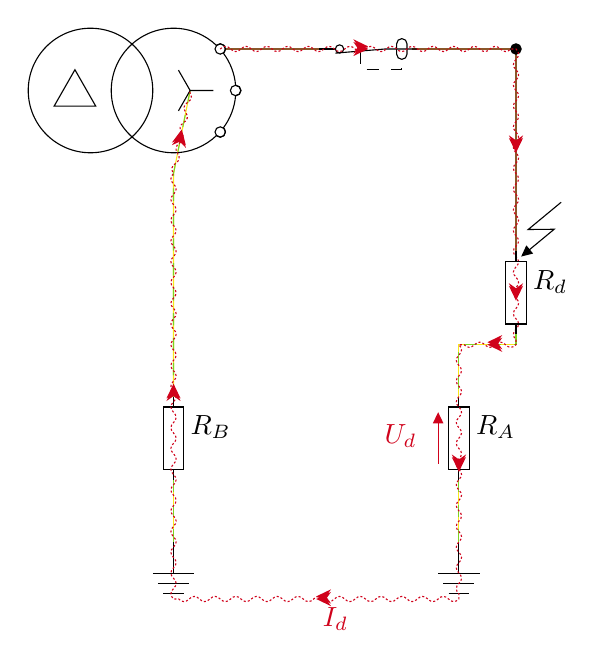
\begin{tikzpicture}[x=0.75pt,y=0.75pt,yscale=-1,xscale=1]
%uncomment if require: \path (0,353); %set diagram left start at 0, and has height of 353

%Straight Lines [id:da8450582290113836] 
\draw [color={rgb, 255:red, 248; green, 231; blue, 28 }  ,draw opacity=1 ]   (87.5,222.5) -- (87.5,252.5) ;
%Straight Lines [id:da035234150750507176] 
\draw [color={rgb, 255:red, 248; green, 231; blue, 28 }  ,draw opacity=1 ]   (252.5,152.5) -- (252.5,157.5) -- (225,157.5) -- (225,182.5) ;
%Straight Lines [id:da575921985906619] 
\draw [color={rgb, 255:red, 139; green, 87; blue, 42 }  ,draw opacity=1 ]   (112.5,15) -- (162.5,15) ;
%Straight Lines [id:da5726536295563455] 
\draw [color={rgb, 255:red, 248; green, 231; blue, 28 }  ,draw opacity=1 ]   (95.5,35) -- (87.5,75) -- (87.5,182.5) ;
%Straight Lines [id:da38476257001275427] 
\draw [color={rgb, 255:red, 126; green, 211; blue, 33 }  ,draw opacity=1 ] [dash pattern={on 4.5pt off 4.5pt}]  (95.5,35) -- (87.5,75) -- (87.5,182.5) ;
%Straight Lines [id:da9973940303994429] 
\draw [color={rgb, 255:red, 139; green, 87; blue, 42 }  ,draw opacity=1 ]   (202.5,15) -- (252.5,15) ;
%Shape: Path Data [id:dp9822778342813306] 
\draw   (112.5,55) .. controls (112.5,56.38) and (111.38,57.5) .. (110,57.5) .. controls (109.29,57.5) and (108.65,57.2) .. (108.19,56.72) .. controls (102.81,61.85) and (95.52,65) .. (87.5,65) .. controls (70.93,65) and (57.5,51.57) .. (57.5,35) .. controls (57.5,18.43) and (70.93,5) .. (87.5,5) .. controls (95.52,5) and (102.81,8.15) .. (108.19,13.28) .. controls (108.65,12.8) and (109.29,12.5) .. (110,12.5) .. controls (111.38,12.5) and (112.5,13.62) .. (112.5,15) .. controls (112.5,15.82) and (112.11,16.54) .. (111.5,17) .. controls (114.8,21.39) and (116.92,26.71) .. (117.4,32.5) .. controls (117.43,32.5) and (117.47,32.5) .. (117.5,32.5) .. controls (118.88,32.5) and (120,33.62) .. (120,35) .. controls (120,36.38) and (118.88,37.5) .. (117.5,37.5) .. controls (117.47,37.5) and (117.43,37.5) .. (117.4,37.5) .. controls (116.92,43.29) and (114.8,48.61) .. (111.5,53) .. controls (112.11,53.46) and (112.5,54.18) .. (112.5,55) -- cycle ;
%Shape: Circle [id:dp10169246549820965] 
\draw   (17.5,35) .. controls (17.5,18.43) and (30.93,5) .. (47.5,5) .. controls (64.07,5) and (77.5,18.43) .. (77.5,35) .. controls (77.5,51.57) and (64.07,65) .. (47.5,65) .. controls (30.93,65) and (17.5,51.57) .. (17.5,35) -- cycle ;
%Shape: Triangle [id:dp22185224755779764] 
\draw   (40,25) -- (30,42.5) -- (50,42.5) -- cycle ;
%Shape: Star [id:dp4535075510124722] 
\draw   (106.75,35) -- (95.5,35) -- (89.88,44.81) -- (95.5,35) -- (89.88,25.19) -- (95.5,35) -- cycle ;
%Shape: Circle [id:dp28187455970704567] 
\draw   (107.5,15) .. controls (107.5,13.62) and (108.62,12.5) .. (110,12.5) .. controls (111.38,12.5) and (112.5,13.62) .. (112.5,15) .. controls (112.5,16.38) and (111.38,17.5) .. (110,17.5) .. controls (108.62,17.5) and (107.5,16.38) .. (107.5,15) -- cycle ;
%Shape: Circle [id:dp9096244123377861] 
\draw   (114.9,35) .. controls (114.9,33.62) and (116.02,32.5) .. (117.4,32.5) .. controls (118.78,32.5) and (119.9,33.62) .. (119.9,35) .. controls (119.9,36.38) and (118.78,37.5) .. (117.4,37.5) .. controls (116.02,37.5) and (114.9,36.38) .. (114.9,35) -- cycle ;
%Shape: Circle [id:dp0660770114066822] 
\draw   (107.5,55) .. controls (107.5,53.62) and (108.62,52.5) .. (110,52.5) .. controls (111.38,52.5) and (112.5,53.62) .. (112.5,55) .. controls (112.5,56.38) and (111.38,57.5) .. (110,57.5) .. controls (108.62,57.5) and (107.5,56.38) .. (107.5,55) -- cycle ;

%Straight Lines [id:da12486709959480935] 
\draw [color={rgb, 255:red, 139; green, 87; blue, 42 }  ,draw opacity=1 ]   (252.5,112.5) -- (252.5,17.5) ;
%Straight Lines [id:da9194886303106931] 
\draw [color={rgb, 255:red, 126; green, 211; blue, 33 }  ,draw opacity=1 ] [dash pattern={on 4.5pt off 4.5pt}]  (252.5,152.5) -- (252.5,157.5) -- (225,157.5) -- (225,182.5) ;
%Straight Lines [id:da33889517147418446] 
\draw    (87.5,252.5) -- (87.5,267.5) ;
%Straight Lines [id:da7536356147270271] 
\draw    (77.5,267.5) -- (97.5,267.5) ;
%Straight Lines [id:da33790733335159795] 
\draw    (80,272.5) -- (95,272.5) ;
%Straight Lines [id:da8225336413065082] 
\draw    (82.5,277.5) -- (92.5,277.5) ;

%Straight Lines [id:da14728368722832463] 
\draw [color={rgb, 255:red, 126; green, 211; blue, 33 }  ,draw opacity=1 ] [dash pattern={on 4.5pt off 4.5pt}]  (87.5,222.5) -- (87.5,252.5) ;
%Straight Lines [id:da2713756434582886] 
\draw [color={rgb, 255:red, 248; green, 231; blue, 28 }  ,draw opacity=1 ]   (225,222.5) -- (225,252.5) ;
%Straight Lines [id:da07200185094723521] 
\draw    (225,252.5) -- (225,267.5) ;
%Straight Lines [id:da5503731135148442] 
\draw    (215,267.5) -- (235,267.5) ;
%Straight Lines [id:da9244125108161202] 
\draw    (217.5,272.5) -- (232.5,272.5) ;
%Straight Lines [id:da07512791048030887] 
\draw    (220,277.5) -- (230,277.5) ;

%Straight Lines [id:da5491926071123034] 
\draw [color={rgb, 255:red, 126; green, 211; blue, 33 }  ,draw opacity=1 ] [dash pattern={on 4.5pt off 4.5pt}]  (225,222.5) -- (225,252.5) ;
%Straight Lines [id:da7705666086878261] 
\draw    (87.5,217.5) -- (87.5,222.5) ;
%Shape: Rectangle [id:dp5724900932521552] 
\draw   (92.5,187.5) -- (92.5,217.5) -- (82.5,217.5) -- (82.5,187.5) -- cycle ;
%Straight Lines [id:da6857493814799358] 
\draw    (87.5,182.5) -- (87.5,187.5) ;

%Straight Lines [id:da7810225170823131] 
\draw    (225,217.5) -- (225,222.5) ;
%Shape: Rectangle [id:dp9839408028922504] 
\draw   (230,187.5) -- (230,217.5) -- (220,217.5) -- (220,187.5) -- cycle ;
%Straight Lines [id:da4367313473487816] 
\draw    (225,182.5) -- (225,187.5) ;

%Shape: Circle [id:dp6401617010113628] 
\draw  [fill={rgb, 255:red, 0; green, 0; blue, 0 }  ,fill opacity=1 ] (250,15) .. controls (250,13.62) and (251.12,12.5) .. (252.5,12.5) .. controls (253.88,12.5) and (255,13.62) .. (255,15) .. controls (255,16.38) and (253.88,17.5) .. (252.5,17.5) .. controls (251.12,17.5) and (250,16.38) .. (250,15) -- cycle ;
%Rounded Rect [id:dp9837999595449706] 
\draw   (197.5,20) .. controls (196.12,20) and (195,18.88) .. (195,17.5) -- (195,12.5) .. controls (195,11.12) and (196.12,10) .. (197.5,10) -- (197.5,10) .. controls (198.88,10) and (200,11.12) .. (200,12.5) -- (200,17.5) .. controls (200,18.88) and (198.88,20) .. (197.5,20) -- cycle ;
%Straight Lines [id:da04140906911364939] 
\draw  [dash pattern={on 4.5pt off 4.5pt}]  (177.5,16) -- (177.5,25) -- (197.5,25) -- (197.5,20) ;
%Shape: Circle [id:dp7012058816599942] 
\draw   (167.5,13) .. controls (166.4,13) and (165.5,13.9) .. (165.5,15) .. controls (165.5,16.1) and (166.4,17) .. (167.5,17) .. controls (168.6,17) and (169.5,16.1) .. (169.5,15) .. controls (169.5,13.9) and (168.6,13) .. (167.5,13) -- cycle ;
%Straight Lines [id:da23692932983683102] 
\draw    (165.5,15) -- (157.5,15) ;
%Straight Lines [id:da4567235518407359] 
\draw    (165.5,17) -- (189.5,15) -- (205,15) ;
%Shape: Boxed Line [id:dp44753967705251496] 
\draw    (274.27,88.83) -- (258.39,101.97) -- (270.89,101.86) -- (257.31,113.09) ;
\draw [shift={(255,115)}, rotate = 320.40999999999997] [fill={rgb, 255:red, 0; green, 0; blue, 0 }  ][line width=0.08]  [draw opacity=0] (5.36,-2.57) -- (0,0) -- (5.36,2.57) -- cycle    ;
\draw [color={rgb, 255:red, 208; green, 2; blue, 27 }  ,draw opacity=1 ] [dash pattern={on 0.75pt off 0.75pt}]  (110,15) .. controls (111.67,13.33) and (113.33,13.33) .. (115,15) .. controls (116.67,16.67) and (118.33,16.67) .. (120,15) .. controls (121.67,13.33) and (123.33,13.33) .. (125,15) .. controls (126.67,16.67) and (128.33,16.67) .. (130,15) .. controls (131.67,13.33) and (133.33,13.33) .. (135,15) .. controls (136.67,16.67) and (138.33,16.67) .. (140,15) .. controls (141.67,13.33) and (143.33,13.33) .. (145,15) .. controls (146.67,16.67) and (148.33,16.67) .. (150,15) .. controls (151.67,13.33) and (153.33,13.33) .. (155,15) .. controls (156.67,16.67) and (158.33,16.67) .. (160,15) .. controls (161.67,13.33) and (163.33,13.33) .. (165,15) .. controls (166.67,16.67) and (168.33,16.67) .. (170,15) .. controls (171.67,13.33) and (173.33,13.33) .. (175,15) .. controls (176.67,16.67) and (178.33,16.67) .. (180,15) .. controls (181.67,13.33) and (183.33,13.33) .. (185,15) .. controls (186.67,16.67) and (188.33,16.67) .. (190,15) .. controls (191.67,13.33) and (193.33,13.33) .. (195,15) .. controls (196.67,16.67) and (198.33,16.67) .. (200,15) .. controls (201.67,13.33) and (203.33,13.33) .. (205,15) .. controls (206.67,16.67) and (208.33,16.67) .. (210,15) .. controls (211.67,13.33) and (213.33,13.33) .. (215,15) .. controls (216.67,16.67) and (218.33,16.67) .. (220,15) .. controls (221.67,13.33) and (223.33,13.33) .. (225,15) .. controls (226.67,16.67) and (228.33,16.67) .. (230,15) .. controls (231.67,13.33) and (233.33,13.33) .. (235,15) .. controls (236.67,16.67) and (238.33,16.67) .. (240,15) .. controls (241.67,13.33) and (243.33,13.33) .. (245,15) .. controls (246.67,16.67) and (248.33,16.67) .. (250,15) -- (252.5,15) -- (252.5,15) .. controls (254.17,16.67) and (254.17,18.33) .. (252.5,20) .. controls (250.83,21.67) and (250.83,23.33) .. (252.5,25) .. controls (254.17,26.67) and (254.17,28.33) .. (252.5,30) .. controls (250.83,31.67) and (250.83,33.33) .. (252.5,35) .. controls (254.17,36.67) and (254.17,38.33) .. (252.5,40) .. controls (250.83,41.67) and (250.83,43.33) .. (252.5,45) .. controls (254.17,46.67) and (254.17,48.33) .. (252.5,50) .. controls (250.83,51.67) and (250.83,53.33) .. (252.5,55) .. controls (254.17,56.67) and (254.17,58.33) .. (252.5,60) .. controls (250.83,61.67) and (250.83,63.33) .. (252.5,65) .. controls (254.17,66.67) and (254.17,68.33) .. (252.5,70) .. controls (250.83,71.67) and (250.83,73.33) .. (252.5,75) .. controls (254.17,76.67) and (254.17,78.33) .. (252.5,80) .. controls (250.83,81.67) and (250.83,83.33) .. (252.5,85) .. controls (254.17,86.67) and (254.17,88.33) .. (252.5,90) .. controls (250.83,91.67) and (250.83,93.33) .. (252.5,95) .. controls (254.17,96.67) and (254.17,98.33) .. (252.5,100) .. controls (250.83,101.67) and (250.83,103.33) .. (252.5,105) .. controls (254.17,106.67) and (254.17,108.33) .. (252.5,110) .. controls (250.83,111.67) and (250.83,113.33) .. (252.5,115) -- (252.5,115) .. controls (254.17,116.67) and (254.17,118.33) .. (252.5,120) .. controls (250.83,121.67) and (250.83,123.33) .. (252.5,125) .. controls (254.17,126.67) and (254.17,128.33) .. (252.5,130) .. controls (250.83,131.67) and (250.83,133.33) .. (252.5,135) .. controls (254.17,136.67) and (254.17,138.33) .. (252.5,140) .. controls (250.83,141.67) and (250.83,143.33) .. (252.5,145) .. controls (254.17,146.67) and (254.17,148.33) .. (252.5,150) .. controls (250.83,151.67) and (250.83,153.33) .. (252.5,155) -- (252.5,157.5) -- (252.5,157.5) .. controls (250.83,159.17) and (249.17,159.17) .. (247.5,157.5) .. controls (245.83,155.83) and (244.17,155.83) .. (242.5,157.5) .. controls (240.83,159.17) and (239.17,159.17) .. (237.5,157.5) .. controls (235.83,155.83) and (234.17,155.83) .. (232.5,157.5) .. controls (230.83,159.17) and (229.17,159.17) .. (227.5,157.5) -- (225,157.5) -- (225,157.5) .. controls (226.67,159.17) and (226.67,160.83) .. (225,162.5) .. controls (223.33,164.17) and (223.33,165.83) .. (225,167.5) .. controls (226.67,169.17) and (226.67,170.83) .. (225,172.5) .. controls (223.33,174.17) and (223.33,175.83) .. (225,177.5) .. controls (226.67,179.17) and (226.67,180.83) .. (225,182.5) .. controls (223.33,184.17) and (223.33,185.83) .. (225,187.5) .. controls (226.67,189.17) and (226.67,190.83) .. (225,192.5) .. controls (223.33,194.17) and (223.33,195.83) .. (225,197.5) .. controls (226.67,199.17) and (226.67,200.83) .. (225,202.5) .. controls (223.33,204.17) and (223.33,205.83) .. (225,207.5) .. controls (226.67,209.17) and (226.67,210.83) .. (225,212.5) .. controls (223.33,214.17) and (223.33,215.83) .. (225,217.5) .. controls (226.67,219.17) and (226.67,220.83) .. (225,222.5) .. controls (223.33,224.17) and (223.33,225.83) .. (225,227.5) .. controls (226.67,229.17) and (226.67,230.83) .. (225,232.5) .. controls (223.33,234.17) and (223.33,235.83) .. (225,237.5) .. controls (226.67,239.17) and (226.67,240.83) .. (225,242.5) .. controls (223.33,244.17) and (223.33,245.83) .. (225,247.5) .. controls (226.67,249.17) and (226.67,250.83) .. (225,252.5) .. controls (223.33,254.17) and (223.33,255.83) .. (225,257.5) .. controls (226.67,259.17) and (226.67,260.83) .. (225,262.5) .. controls (223.33,264.17) and (223.33,265.83) .. (225,267.5) .. controls (226.67,269.17) and (226.67,270.83) .. (225,272.5) .. controls (223.33,274.17) and (223.33,275.83) .. (225,277.5) -- (225,280) -- (225,280) .. controls (223.33,281.67) and (221.67,281.67) .. (220,280) .. controls (218.33,278.33) and (216.67,278.33) .. (215,280) .. controls (213.33,281.67) and (211.67,281.67) .. (210,280) .. controls (208.33,278.33) and (206.67,278.33) .. (205,280) .. controls (203.33,281.67) and (201.67,281.67) .. (200,280) .. controls (198.33,278.33) and (196.67,278.33) .. (195,280) .. controls (193.33,281.67) and (191.67,281.67) .. (190,280) .. controls (188.33,278.33) and (186.67,278.33) .. (185,280) .. controls (183.33,281.67) and (181.67,281.67) .. (180,280) .. controls (178.33,278.33) and (176.67,278.33) .. (175,280) .. controls (173.33,281.67) and (171.67,281.67) .. (170,280) .. controls (168.33,278.33) and (166.67,278.33) .. (165,280) .. controls (163.33,281.67) and (161.67,281.67) .. (160,280) .. controls (158.33,278.33) and (156.67,278.33) .. (155,280) .. controls (153.33,281.67) and (151.67,281.67) .. (150,280) .. controls (148.33,278.33) and (146.67,278.33) .. (145,280) .. controls (143.33,281.67) and (141.67,281.67) .. (140,280) .. controls (138.33,278.33) and (136.67,278.33) .. (135,280) .. controls (133.33,281.67) and (131.67,281.67) .. (130,280) .. controls (128.33,278.33) and (126.67,278.33) .. (125,280) .. controls (123.33,281.67) and (121.67,281.67) .. (120,280) .. controls (118.33,278.33) and (116.67,278.33) .. (115,280) .. controls (113.33,281.67) and (111.67,281.67) .. (110,280) .. controls (108.33,278.33) and (106.67,278.33) .. (105,280) .. controls (103.33,281.67) and (101.67,281.67) .. (100,280) .. controls (98.33,278.33) and (96.67,278.33) .. (95,280) .. controls (93.33,281.67) and (91.67,281.67) .. (90,280) -- (87.5,280) -- (87.5,280) .. controls (85.83,278.33) and (85.83,276.67) .. (87.5,275) .. controls (89.17,273.33) and (89.17,271.67) .. (87.5,270) .. controls (85.83,268.33) and (85.83,266.67) .. (87.5,265) .. controls (89.17,263.33) and (89.17,261.67) .. (87.5,260) .. controls (85.83,258.33) and (85.83,256.67) .. (87.5,255) .. controls (89.17,253.33) and (89.17,251.67) .. (87.5,250) .. controls (85.83,248.33) and (85.83,246.67) .. (87.5,245) .. controls (89.17,243.33) and (89.17,241.67) .. (87.5,240) .. controls (85.83,238.33) and (85.83,236.67) .. (87.5,235) .. controls (89.17,233.33) and (89.17,231.67) .. (87.5,230) .. controls (85.83,228.33) and (85.83,226.67) .. (87.5,225) .. controls (89.17,223.33) and (89.17,221.67) .. (87.5,220) .. controls (85.83,218.33) and (85.83,216.67) .. (87.5,215) .. controls (89.17,213.33) and (89.17,211.67) .. (87.5,210) .. controls (85.83,208.33) and (85.83,206.67) .. (87.5,205) .. controls (89.17,203.33) and (89.17,201.67) .. (87.5,200) .. controls (85.83,198.33) and (85.83,196.67) .. (87.5,195) .. controls (89.17,193.33) and (89.17,191.67) .. (87.5,190) .. controls (85.83,188.33) and (85.83,186.67) .. (87.5,185) .. controls (89.17,183.33) and (89.17,181.67) .. (87.5,180) .. controls (85.83,178.33) and (85.83,176.67) .. (87.5,175) .. controls (89.17,173.33) and (89.17,171.67) .. (87.5,170) .. controls (85.83,168.33) and (85.83,166.67) .. (87.5,165) .. controls (89.17,163.33) and (89.17,161.67) .. (87.5,160) .. controls (85.83,158.33) and (85.83,156.67) .. (87.5,155) .. controls (89.17,153.33) and (89.17,151.67) .. (87.5,150) .. controls (85.83,148.33) and (85.83,146.67) .. (87.5,145) .. controls (89.17,143.33) and (89.17,141.67) .. (87.5,140) .. controls (85.83,138.33) and (85.83,136.67) .. (87.5,135) .. controls (89.17,133.33) and (89.17,131.67) .. (87.5,130) .. controls (85.83,128.33) and (85.83,126.67) .. (87.5,125) .. controls (89.17,123.33) and (89.17,121.67) .. (87.5,120) .. controls (85.83,118.33) and (85.83,116.67) .. (87.5,115) .. controls (89.17,113.33) and (89.17,111.67) .. (87.5,110) .. controls (85.83,108.33) and (85.83,106.67) .. (87.5,105) .. controls (89.17,103.33) and (89.17,101.67) .. (87.5,100) .. controls (85.83,98.33) and (85.83,96.67) .. (87.5,95) .. controls (89.17,93.33) and (89.17,91.67) .. (87.5,90) .. controls (85.83,88.33) and (85.83,86.67) .. (87.5,85) .. controls (89.17,83.33) and (89.17,81.67) .. (87.5,80) .. controls (85.83,78.33) and (85.83,76.67) .. (87.5,75) -- (87.5,75) .. controls (86.19,73.04) and (86.52,71.41) .. (88.48,70.1) .. controls (90.44,68.79) and (90.77,67.15) .. (89.46,65.19) .. controls (88.15,63.23) and (88.48,61.6) .. (90.44,60.29) .. controls (92.4,58.98) and (92.73,57.35) .. (91.42,55.39) .. controls (90.11,53.43) and (90.44,51.8) .. (92.4,50.49) .. controls (94.36,49.18) and (94.69,47.54) .. (93.38,45.58) .. controls (92.07,43.62) and (92.4,41.99) .. (94.36,40.68) .. controls (96.32,39.37) and (96.65,37.74) .. (95.34,35.78) -- (95.5,35) -- (95.5,35) ;
\draw [shift={(181.25,15)}, rotate = 180] [fill={rgb, 255:red, 208; green, 2; blue, 27 }  ,fill opacity=1 ][line width=0.08]  [draw opacity=0] (7.14,-3.43) -- (0,0) -- (7.14,3.43) -- (4.74,0) -- cycle    ;
\draw [shift={(252.5,65)}, rotate = 270] [fill={rgb, 255:red, 208; green, 2; blue, 27 }  ,fill opacity=1 ][line width=0.08]  [draw opacity=0] (7.14,-3.43) -- (0,0) -- (7.14,3.43) -- (4.74,0) -- cycle    ;
\draw [shift={(252.5,136.25)}, rotate = 270] [fill={rgb, 255:red, 208; green, 2; blue, 27 }  ,fill opacity=1 ][line width=0.08]  [draw opacity=0] (7.14,-3.43) -- (0,0) -- (7.14,3.43) -- (4.74,0) -- cycle    ;
\draw [shift={(238.75,157.5)}, rotate = 360] [fill={rgb, 255:red, 208; green, 2; blue, 27 }  ,fill opacity=1 ][line width=0.08]  [draw opacity=0] (7.14,-3.43) -- (0,0) -- (7.14,3.43) -- (4.74,0) -- cycle    ;
\draw [shift={(225,218.75)}, rotate = 270] [fill={rgb, 255:red, 208; green, 2; blue, 27 }  ,fill opacity=1 ][line width=0.08]  [draw opacity=0] (7.14,-3.43) -- (0,0) -- (7.14,3.43) -- (4.74,0) -- cycle    ;
\draw [shift={(156.25,280)}, rotate = 360] [fill={rgb, 255:red, 208; green, 2; blue, 27 }  ,fill opacity=1 ][line width=0.08]  [draw opacity=0] (7.14,-3.43) -- (0,0) -- (7.14,3.43) -- (4.74,0) -- cycle    ;
\draw [shift={(87.5,177.5)}, rotate = 450] [fill={rgb, 255:red, 208; green, 2; blue, 27 }  ,fill opacity=1 ][line width=0.08]  [draw opacity=0] (7.14,-3.43) -- (0,0) -- (7.14,3.43) -- (4.74,0) -- cycle    ;
\draw [shift={(91.5,55)}, rotate = 461.31] [fill={rgb, 255:red, 208; green, 2; blue, 27 }  ,fill opacity=1 ][line width=0.08]  [draw opacity=0] (7.14,-3.43) -- (0,0) -- (7.14,3.43) -- (4.74,0) -- cycle    ;
\draw [shift={(181.25,13.75)}, rotate = 180] [fill={rgb, 255:red, 208; green, 2; blue, 27 }  ,fill opacity=1 ][line width=0.08]  [draw opacity=0] (7.14,-3.43) -- (0,0) -- (7.14,3.43) -- (4.74,0) -- cycle    ;
\draw [shift={(252.5,63.75)}, rotate = 270] [fill={rgb, 255:red, 208; green, 2; blue, 27 }  ,fill opacity=1 ][line width=0.08]  [draw opacity=0] (7.14,-3.43) -- (0,0) -- (7.14,3.43) -- (4.74,0) -- cycle    ;
\draw [shift={(252.5,135)}, rotate = 270] [fill={rgb, 255:red, 208; green, 2; blue, 27 }  ,fill opacity=1 ][line width=0.08]  [draw opacity=0] (7.14,-3.43) -- (0,0) -- (7.14,3.43) -- (4.74,0) -- cycle    ;
\draw [shift={(238.75,156.25)}, rotate = 360] [fill={rgb, 255:red, 208; green, 2; blue, 27 }  ,fill opacity=1 ][line width=0.08]  [draw opacity=0] (7.14,-3.43) -- (0,0) -- (7.14,3.43) -- (4.74,0) -- cycle    ;
\draw [shift={(225,217.5)}, rotate = 270] [fill={rgb, 255:red, 208; green, 2; blue, 27 }  ,fill opacity=1 ][line width=0.08]  [draw opacity=0] (7.14,-3.43) -- (0,0) -- (7.14,3.43) -- (4.74,0) -- cycle    ;
\draw [shift={(156.25,278.75)}, rotate = 360] [fill={rgb, 255:red, 208; green, 2; blue, 27 }  ,fill opacity=1 ][line width=0.08]  [draw opacity=0] (7.14,-3.43) -- (0,0) -- (7.14,3.43) -- (4.74,0) -- cycle    ;
\draw [shift={(87.5,176.25)}, rotate = 450] [fill={rgb, 255:red, 208; green, 2; blue, 27 }  ,fill opacity=1 ][line width=0.08]  [draw opacity=0] (7.14,-3.43) -- (0,0) -- (7.14,3.43) -- (4.74,0) -- cycle    ;
\draw [shift={(91.5,53.75)}, rotate = 461.31] [fill={rgb, 255:red, 208; green, 2; blue, 27 }  ,fill opacity=1 ][line width=0.08]  [draw opacity=0] (7.14,-3.43) -- (0,0) -- (7.14,3.43) -- (4.74,0) -- cycle    ;
%Straight Lines [id:da9207949526828273] 
\draw    (252.5,147.5) -- (252.5,152.5) ;
%Shape: Rectangle [id:dp36210266951689685] 
\draw   (257.5,117.5) -- (257.5,147.5) -- (247.5,147.5) -- (247.5,117.5) -- cycle ;
%Straight Lines [id:da2843419817195654] 
\draw    (252.5,112.5) -- (252.5,117.5) ;

%Straight Lines [id:da667113945803525] 
\draw [color={rgb, 255:red, 208; green, 2; blue, 27 }  ,draw opacity=1 ]   (215,193) -- (215,215) ;
\draw [shift={(215,190)}, rotate = 90] [fill={rgb, 255:red, 208; green, 2; blue, 27 }  ,fill opacity=1 ][line width=0.08]  [draw opacity=0] (5.36,-2.57) -- (0,0) -- (5.36,2.57) -- cycle    ;

% Text Node
\draw (94.5,190.5) node [anchor=north west][inner sep=0.75pt]   [align=left] {$R_B$};
% Text Node
\draw (232,190.5) node [anchor=north west][inner sep=0.75pt]   [align=left] {$R_A$};
% Text Node
\draw (188,194.5) node [anchor=north west][inner sep=0.75pt]  [color={rgb, 255:red, 208; green, 2; blue, 27 }  ,opacity=1 ] [align=left] {$U_d$};
% Text Node
\draw (259.5,120.5) node [anchor=north west][inner sep=0.75pt]   [align=left] {$R_d$};
% Text Node
\draw (158.25,283) node [anchor=north west][inner sep=0.75pt] [color={rgb, 255:red, 208; green, 2; blue, 27 }]  [align=left] {$I_d$};


\end{tikzpicture}

\end{figure}

%\end{document}


\begin{comment}
\begin{circuitikz}[circuit ee IEC relay]
%\DrawGrid{(-1,-5)}{(9,3)} %grille d'aide pour le placement des objets

%alimentation

\node (D1) [make contact=point left, circuit breaker={point left}, tiny circuit symbols, activated] at (1,0.45) {};
\node (T1) [oosourcetransshape, prim=delta,sec=wye] at (0,0) {};


%neutre/terre

\node (RN) [R, label=$R_B$, rotate=90, tiny circuit symbols] at (0,-2.7) {};
\node (G1) [tlground] at (0,-3.9) {};
\draw [green!, thick] (G1) to node {} (RN) ; 
\draw [green!, thick] (RN) to (0,-0.5) to node {} (T1.sec4) ; 
\draw [dashed, yellow!, thick] (G1) to node {} (RN) ;
\draw [dashed, yellow!, thick] (RN) to (0,-0.5) to node {} (T1.sec4) ;

\node (RT) [resistor, rotate=90, tiny circuit symbols, label=$R_A$] at (2.5,-2.7) {};
\draw[-triangle 45, red] (2.8,-2) -- (2.8,-1) node[right,midway] {$U_d$};
\node (G2) [tlground] at (2.5,-3.9) {};
\draw [green!, thick] (RT) to (G2); 
\draw [dashed, yellow!, thick] (RT) to (G2);
\node (G2) [tlground] at (2.5,-3.9) {};
\draw [green!, thick] (G1) to (0,-4.2) to (2.5,-4.2) to (G2);
\draw [dashed, yellow!, thick] (G1) -- (0,-4.2) -- (2.5,-4.2) node [midway,below] {\color{black}$I_d$} -- (G2);
\node (G1) [tlground] at (0,-3.9) {};
\node (G2) [tlground] at (2.5,-3.9) {};

%appareil 1

\node (C2) [circ, scale=0.5] at (2.5,0.45) {};
\node (RD) [resistor, label=$R_d$, rotate=90, tiny circuit symbols] at (2.5,-1.5) {};

\draw [green!, thick] (RD) to (RT); 
\draw [dashed, yellow!, thick] (RD) to (RT); 

\draw [brown, thick] (T1.sec1) to (0.5,0.45) to (D1) to (C2) to (RD);
\node (T1) [oosourcetransshape, prim=delta,sec=wye] at (0,0) {};

%chemin courant

\fill [yellow!, decoration=lightning bolt, decorate] (2.5,-1.2) -- ++ (0.5,0.8); %éclairs
\path [postaction={on each segment={mid arrow=red}}]  (T1.sec1) -- (0.5,0.45) -- (D1) -- (C2) -- (RD) -- (RT) -- (G2) -- (2.5,-4.2) -- (1.666,-4.2) -- (0.88888,-4.2)  -- (0,-4.2) -- (G1) -- (RN) -- (0,-0.5) -- (T1.sec4); 

\callout{1,-0.5}{\cstep\label{pas:1}}{2.4,-1.2};


\end{circuitikz}
\end{comment}


L'intensité de courant $I_d$ vaut alors :
\begin{formule}[Courant de défaut $I_d$ en schéma TT]
\begin{align*}
		I_d &= \frac{U_{0}}{R_{B}+R_{A}+R_{d}}
\end{align*}
\end{formule}

\begin{textvariables}
U_{0}						& tension nominale simple						& volt			& \volt					& 	Différence de potentiel entre les masses métalliques et la terre 	\\
R_{B}						& résistance						& ohm			& \ohm					& 	Résistance de la prise de terre du neutre 	\\
R_{A}						& résistance						& ohm			& \ohm					& 	Résistance de la prise de terre de l'installation électrique 	\\
R_{d}						& résistance						& ohm			& \ohm					& 	Résistance de défaut 	d'isolement \\
\end{textvariables}

Le courant de défaut $I_d$ fera alors apparaître une \emph{tension de défaut} $U_d$ entre la masse métallique et la terre. Pour satisfaire aux normes de sécurité de la NF C15-100, il est imposé que la tension de défaut $U_d$ ne dépasse pas la tension de sécurité du local $U_L$ (voir \superref{subsec:prise_terre_installation_electrique}) :

\begin{formule}[Tension de défaut $U_d$ en schéma TT]
\begin{align*}
		U_d &= R_{A} \times I_{d} \\
			   &< U_L
\end{align*}
\end{formule}

\begin{textvariables}
R_{A}						& résistance						& ohm			& \ohm					& 	Résistance de la prise de terre de l'installation électrique 	\\
I_{d}							& intensité							& ampère		& \ampere				& 	Courant de défaut d'isolement \\
U_{L}						& tension							& volt			& \volt					& 	Tension de sécurité du local avec :
\begin{description}[nosep, leftmargin=*]
\item[Local sec :] $U_{L}=\SI{50}{\volt}$
\item[Local humide :] $U_{L}=\SI{25}{\volt}$
\end{description} \\
\end{textvariables}

Il est donc nécessaire de limiter $U_d$ à la valeur suivante (voir \superref{form:resistance_prise_terre}) :

\begin{formule}[Calibre du DDR $I_{\Delta n}$]
\begin{align*}
		I_{\Delta n} &< \frac{U_{L}}{R_{A}}
\end{align*}
\end{formule}

\begin{textvariables}
U_{L}						& tension							& volt			& \volt					& 	Tension de sécurité du local avec :
\begin{description}[nosep, leftmargin=*]
\item[Local sec :] $U_{L}=\SI{50}{\volt}$
\item[Local humide :] $U_{L}=\SI{25}{\volt}$
\end{description} \\
R_{A}						& résistance						& ohm			& \ohm					& 	Résistance de la prise de terre de l'installation électrique 	\\
\end{textvariables}

\begin{exemple}[Calcul du calibre du DDR $I_{\Delta n}$]
Si on considère que le transformateur est un transformateur $\SI{20}{\kilo\volt}/\SI{400}{\volt}$, que $R_A=\SI{20}{\ohm}$, que $R_B=\SI{10}{\ohm}$ et que $R_d$ est négligée, on peut déduire que le courant de défaut $I_d$ vaut :
\begin{align*}
		I_d 	&= \frac{U_{0}}{R_{B}+R_{A}} \\
				&=\frac{400}{20+10} \\
				&= \SI{13,33}{\ampere} \\
\end{align*}
Si une personne touche une masse des récepteurs en défaut, elle sera soumise à une tension de défaut $U_d$ :
\begin{align*}
		U_d 	&= R_{A} \times I_{d} \\
				&=20 \times 13,33 \\
				&= \SI{266,6}{\volt}
\end{align*}
La tension de défaut $U_d$ est dangereuse quelle que soit la tension limite choisie :
\begin{itemize}
\item coupure la plus rapide possible\,;
\item protection des personnes.
\end{itemize}
~\\
\begin{minipage}[t]{0.5\linewidth}
Dans le cas d'un local sec :
\begin{align*}
	I_{\Delta n} 	&< \frac{U_{L}}{R_{A}} \\
						&< \frac{50}{20} \\
						&< \SI{2,5}{\ampere}
\end{align*}
\end{minipage}
\hfill
\begin{minipage}[t]{0.5\linewidth}
Dans le cas d'un local humide :
\begin{align*}
	I_{\Delta n} 	&< \frac{U_{L}}{R_{A}} \\
						&< \frac{25}{20} \\
						&< \SI{1,25}{\ampere}
\end{align*}
\end{minipage}
~\\
D'après le tableau situé en \superref{tab:temps_coupure_DDR}, le DDR doit présenter un temps de coupure de moins de \SI{70}{\milli\second} avec une tension de défaut $U_d$ de \SI{266,6}{\volt} :

\begin{table}[h]
\begin{tabularx}{\linewidth}{X cccccccc}
\toprule
Tension nominale		& \multicolumn{2}{c}{$\SI{50}{\volt}<U_0\leq\SI{120}{\volt}$} 	& \multicolumn{2}{c}{$\SI{120}{\volt}<U_0\leq\SI{230}{\volt}$} & \multicolumn{2}{c}{$\SI{230}{\volt}<U_0\leq\SI{400}{\volt}$}		& \multicolumn{2}{c}{$U_0>\SI{400}{\volt}$}\\
\midrule
Type de courant		& alternatif	& continu	& alternatif	& continu	& alternatif	& continu	& alternatif	& continu \\
\addlinespace
Schéma TN/IT	& \SI{0,8}{\second}	&	\SI{5}{\second}	&	\SI{0,4}{\second}	&	\SI{5}{\second}	&	\SI{0,2}{\second}	&	\SI{0,4}{\second}	&	\SI{0,1}{\second}	&	\SI{0,1}{\second} \\	
\addlinespace
Schéma TT	& \SI{0,3}{\second}	&	\SI{5}{\second}	&	\SI{0,2}{\second}	&	\SI{0,4}{\second}	&	\cellcolor{green}\SI{0,07}{\second}	&	\SI{0,2}{\second}	&	\SI{0,04}{\second}	&	\SI{0,1}{\second} \\	
\bottomrule
\end{tabularx}
\end{table}
\end{exemple}

%\end{document}
